\documentclass[letterpaper, 12pt]{article}

% \usepackage[showframe, margin=1in, top=0.25in, bottom=0.25in, includeheadfoot, headheight=0.5in]{geometry}
\usepackage[margin=1in, top=0.25in, bottom=0.25in, includeheadfoot, headheight=0.5in]{geometry}

\AddToHook{cmd/section/before}{\clearpage}

\usepackage[table]{xcolor}
\colorlet{listingback}{gray!20}
\definecolor{headingcolor}{RGB}{110,34,54}

\usepackage{fancyhdr}
\renewcommand{\sectionmark}[1]{\markboth{#1}{#1}}

% Used to detect whether a section is an appendix to print the right thing in the footer
\usepackage{etoolbox}
\newtoggle{inappendix}
\pretocmd{\appendix}{\clearpage\toggletrue{inappendix}}{}{}

% Save standard definitions for head and foot rules (lines separating header and footer from text)
\let\HeadRule\headrule
\let\FootRule\footrule
% Add color to the standard definitions
\renewcommand{\headrule}{\color{headingcolor}\HeadRule}
\renewcommand{\footrule}{\textcolor{headingcolor}{\FootRule}}

% IMPORTANT: This command should not be called directly. Use \preamble.
% Macro to insert the title page for each lab.
% The argument is the title of the lab.
\newcommand{\inserttitlepage}[1]
{
    \begin{titlepage}
    \centering
    
\includegraphics[scale=0.5]{images/nexus_lab_logo.png}

    \vspace*{\baselineskip}

    \textbf{\Large OpenStack Labs}

    \vspace*{\baselineskip}

    \textbf{\Large #1}
    \vspace*{\fill}
\end{titlepage}
}

% IMPORTANT: This command should not be called directly. Use \preamble.
% Macro to define header and footer for each lab.
% The argument is the title of the lab.
\newcommand{\headfoot}[1]
{
    \fancypagestyle{fancy}
    {
        \fancyhf{}
        \fancyhead[L]{\footnotesize #1}
        \fancyhead[R]{
\includegraphics[height=0.85\headheight]{images/nexus_lab_logo.png}}
        \fancyfoot[L]{%
            \footnotesize%
            \ifnum\value{section}>0%
            \iftoggle{inappendix}{Appendix \thesection: \rightmark}{Section \thesection: \rightmark}%
            \fi}
        \fancyfoot[R]{\footnotesize\thepage}
        \renewcommand{\headrulewidth}{1.5pt}
        \renewcommand{\footrulewidth}{1.5pt}
    }
}

% Macro to insert title page, define header and footer, and insert table of contents and about section for each lab.
% The argument is the title of the lab.
\newcommand{\preamble}[1]
{
    \pagenumbering{roman}
    \inserttitlepage{#1}
    \headfoot{#1}

    % Insert table of contents
    \pagestyle{fancy}
    \tableofcontents
    \clearpage

    \section*{About This Document}
    \label{sec:about_this_document}
    \begin{itemize}
        \item This document was developed by a team at the University of Tennessee at Chattanooga led by Dr. Mengjun Xie
        (\href{mailto:mengjun-xie@utc.edu}{\textbf{mengjun-xie@utc.edu}}).
        \item The development of this document was supported by a National Centers of Academic Excellence in Cybersecurity Grant (\#H98230-20-1-0351), housed at the National Security Agency.
        \item This document is licensed with a Creative Commons Attribution 4.0 International License.
    \end{itemize}
    \clearpage
}

% Macro to insert the Lab Settings page for each lab. Call after the Introduction and Objectives sections.
\newcommand{\labsettings}
{
    \section*{Lab Settings}
    \label{sec:lab_settings}
    \addcontentsline{toc}{section}{\nameref{sec:lab_settings}}
    The information in the table below will be needed in order to complete the lab.
    The task sections below provide details on the use of this information.
    \begin{table*}[htbp]
        \centering
        \begin{tabular}{|c|c|c|c|}
            \hline
            \rowcolor{gray!20} \textbf{Virtual Machine} & \textbf{IP Address} & \textbf{Account} & \textbf{Password} \\
            \hline
            \multirow{2}{*}{\texttt{workstation}} & \multirow[t]{2}{*}{\texttt{ens3: 192.168.1.21}}  & \multirow{2}{*}{\texttt{ubuntu}} & \multirow{2}{*}{\texttt{ubuntu}} \\
                                                  & \multirow[t]{2}{*}{\texttt{ens4: 172.25.250.21}} &                                  &                                  \\
            \hline
            \multirow{2}{*}{\texttt{devstack}}    & \multirow[t]{2}{*}{\texttt{ens3: 192.168.20}}    & \multirow{2}{*}{\texttt{ubuntu}} & \multirow{2}{*}{\texttt{ubuntu}} \\
                                                  & \multirow[t]{2}{*}{\texttt{ens4: 172.25.250.20}} &                                  &                                  \\
            \hline
        \end{tabular}
    \end{table*}
    \clearpage

    % IMPORTANT(lucas): If another frontmatter section ever gets placed after this, this command needs to be moved
    % to the end of that section.
    % I have placed this here and not in each lab purely for convenience and to ensure I don't forget any.
    \pagenumbering{arabic}
}

% Sans-serif font
\renewcommand{\familydefault}{\sfdefault}
\newcommand{\texttildemid}{{\raisebox{0.5ex}{\texttildelow}}}

\usepackage{enumitem}
\renewcommand{\labelenumi}{\textbf{\thesection.\arabic{enumi}.}}

% Try to forbid widows and orphans
\widowpenalty10000
\clubpenalty10000

\usepackage{graphicx}
\usepackage{hyperref}
\hypersetup{colorlinks=true,linkcolor=black,urlcolor={[named] headingcolor}}

\usepackage{sectsty}
\sectionfont{\color{headingcolor}}

% Table of Contents
\usepackage{bookmark}
\usepackage[titles]{tocloft}
\usepackage[title]{appendix}
\renewcommand{\cfttoctitlefont}{\Large\bfseries\color{headingcolor}}
\renewcommand{\cftsecfont}{\normalfont\normalsize}
\renewcommand{\cftsecpagefont}{\normalfont\normalsize}
\renewcommand{\cftdotsep}{0} % Make dots small and close together
\renewcommand{\cftsecleader}{\cftdotfill{\cftdotsep}} % Add dots after section titles
% Make dots go all the way to the page number
\renewcommand{\cftsecfillnum}[1]{{\cftsecleader}\nobreak{\cftsecpagefont #1}\cftsecafterpnum\par}

\usepackage{multirow}
\setlength{\tabcolsep}{16pt}
\renewcommand{\arraystretch}{1.1}

% For nice-looking boxes
\usepackage[most]{tcolorbox}
\usepackage{listings}
\usepackage{lstautogobble}
\lstset{
  frame=none,
  language=Bash,
  showstringspaces=false,
  basicstyle={\linespread{1.1}\footnotesize\ttfamily\selectfont},
  numbers=none,
  breaklines=true,
  breakatwhitespace=true,
  tabsize=3,
  columns=fullflexible,
  keepspaces=true,
  escapeinside={(*@}{@*)},
  literate={~}{{\texttildemid}}{1}
           {\#}{\#}{1},
  autogobble=true
}

\tcolorboxenvironment{lstlisting}
{
    spartan,
    colframe=gray!50,
    boxsep=0mm,
    left=1mm,
    right=1mm,
    top=-1mm,
    bottom=-1mm,
    colback=gray!20
}

% Hacky solution for now, would like to have just one environment and make several tcolorboxes by passing different
% colors as parameters, but that is giving errors
\makeatletter
\tcbset{
  note/.style={%
        enhanced,
        breakable,
        colback=blue!10!white,
        colframe=blue!80!white,
        attach boxed title to top left={yshift*=-\tcboxedtitleheight},
        title={#1},
        boxed title size=title,
        boxed title style={%
            sharp corners,
            rounded corners=northwest,
            colback=tcbcolframe,
            boxrule=0pt,
        },
        underlay boxed title={%
            \path[fill=tcbcolframe] (title.south west)--(title.south east)
                to[out=0, in=180] ([xshift=5mm]title.east)--
                (title.center-|frame.east)
                [rounded corners=\kvtcb@arc] |-
                (frame.north) -| cycle;
        },
    }
}
\makeatother

\makeatletter
\tcbset{
    stop/.style={%
        enhanced,
        breakable,
        colback=white,
        colback=red!10!white,
        colframe=red!80!white,
        attach boxed title to top left={yshift*=-\tcboxedtitleheight},
        title={#1},
        boxed title size=title,
        boxed title style={%
            sharp corners,
            rounded corners=northwest,
            colback=tcbcolframe,
            boxrule=0pt,
        },
        underlay boxed title={%
            \path[fill=tcbcolframe] (title.south west)--(title.south east)
                to[out=0, in=180] ([xshift=5mm]title.east)--
                (title.center-|frame.east)
                [rounded corners=\kvtcb@arc] |-
                (frame.north) -| cycle;
        },
    }
}
\makeatother

\makeatletter
\tcbset{
    tip/.style={%
        enhanced,
        breakable,
        colback=white,
        colback=green!10,
        colframe=green!70!black,
        attach boxed title to top left={yshift*=-\tcboxedtitleheight},
        fonttitle=\bfseries,
        title={#1},
        boxed title size=title,
        boxed title style={%
            sharp corners,
            rounded corners=northwest,
            colback=tcbcolframe,
            boxrule=0pt,
        },
        underlay boxed title={%
            \path[fill=tcbcolframe] (title.south west)--(title.south east)
                to[out=0, in=180] ([xshift=5mm]title.east)--
                (title.center-|frame.east)
                [rounded corners=\kvtcb@arc] |-
                (frame.north) -| cycle;
        },
    }
}
\makeatother

% The commands below define environments for colored boxes. They are used like
% \begin{notebox}
% ...
% \end{notebox}
\newtcolorbox{notebox}{note={Note}}
\newtcolorbox{stopbox}{stop={Stop}}
\newtcolorbox{tipbox}{tip={Tip}}


\begin{document}

\preamble{Lab 03: Deploying an Internal Instance}

\section*{Introduction}
\label{sec:introduction}
\addcontentsline{toc}{section}{\nameref{sec:introduction}}
In this lab, you will manage images using the \textit{Horizon Dashboard} and \textit{OpenStack Unified CLI}, develop
flavors, manage private networks, launch an internal instance, and verify the functionality of an internal instance.

\section*{Objectives}
\label{sec:objectives}
\addcontentsline{toc}{section}{\nameref{sec:objectives}}
\begin{itemize}[itemsep=0pt]
    \item Manage software profiles (images)
    \item Manage hardware profiles (flavors)
    \item Manage private networks
    \item Launch and verify an internal instance
\end{itemize}

\labsettings

%%%%%%%%%%%
% Section 1
%%%%%%%%%%%
\section{Uploading Images}
\label{sec:uploading_images}
In this task, you will create, modify, and delete images using the \textit{Horizon Dashboard} and
\textit{OpenStack Unified CLI}.

\begin{enumerate}
    \item Log into the \textbf{workstation} machine as the \textbf{ubuntu} user with password \textbf{ubuntu}.

    \begin{center}
        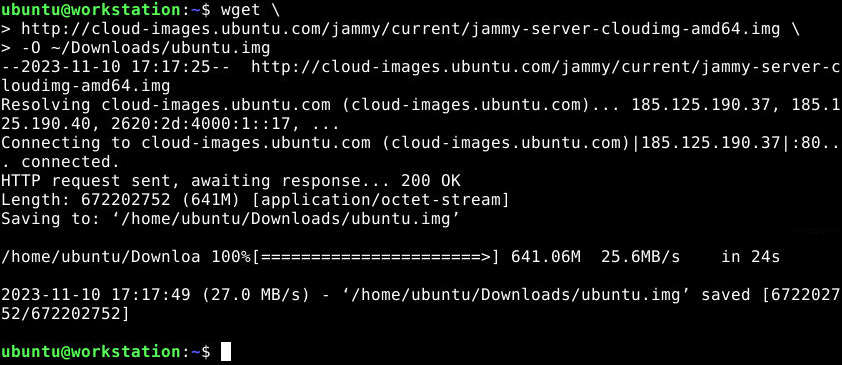
\includegraphics[width=\linewidth]{images/part1/step1.png}
    \end{center}

    \item Launch the graphical user interface.
    \begin{lstlisting}
        ubuntu@workstation:~$ startx
    \end{lstlisting}

    \begin{center}
        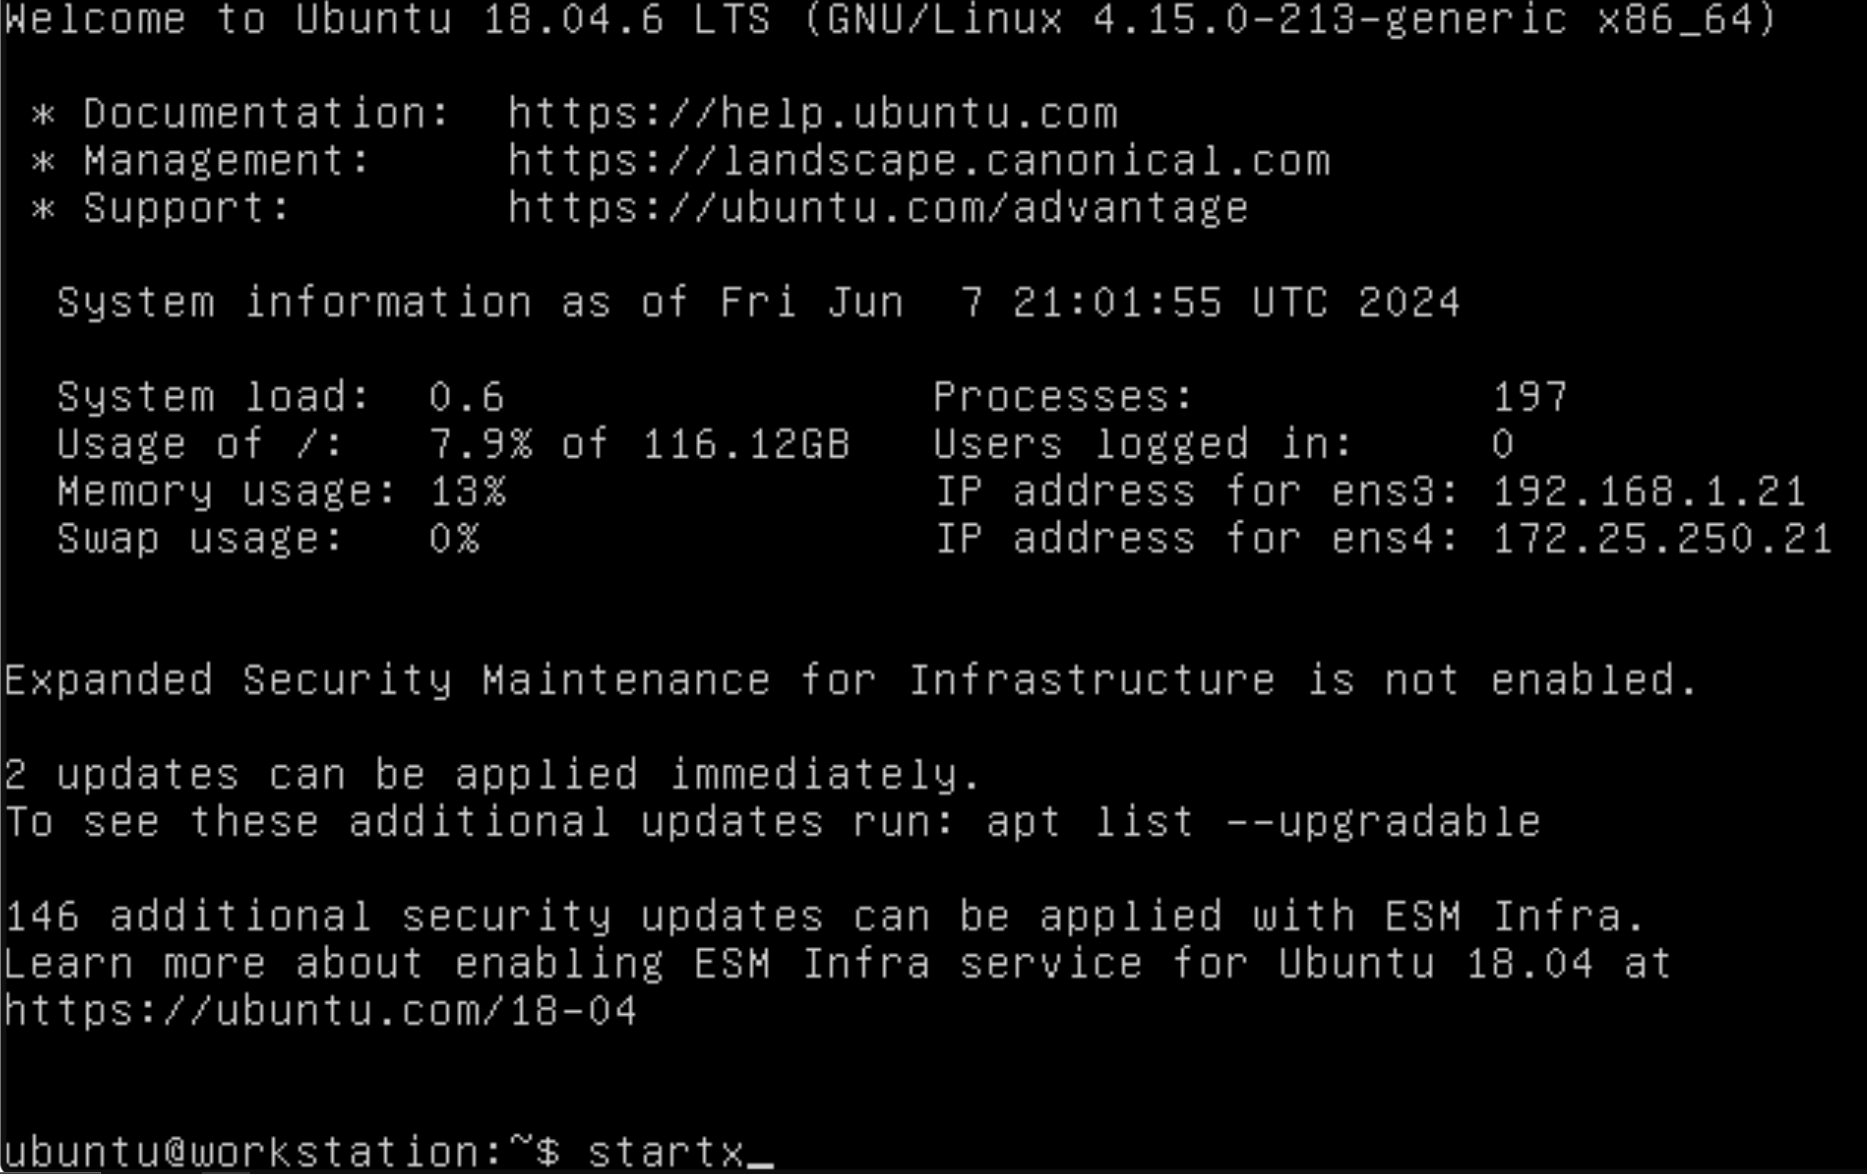
\includegraphics[width=\linewidth]{images/part1/step2.png}
    \end{center}

    \item Open the web browser. Navigate to \textbf{192.168.1.20} and log into the dashboard as \textbf{admin} with the
    password \textbf{secret}.

    \item Switch to the \textbf{demo} project. In this lab, we will create our own Ubuntu images, so the default one is
    not needed and can be deleted. Navigate to \textbf{Project $>$ Compute $>$ Images}. Select the \textbf{ubuntu} image
    and click \textbf{Delete Image}.

    \begin{center}
        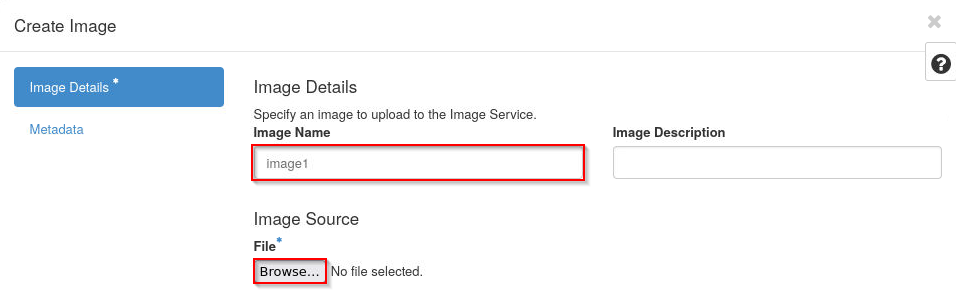
\includegraphics[width=\linewidth]{images/part1/step4.png}
    \end{center}

    \item Click \textbf{Create Image} to create a new image.

    \begin{center}
        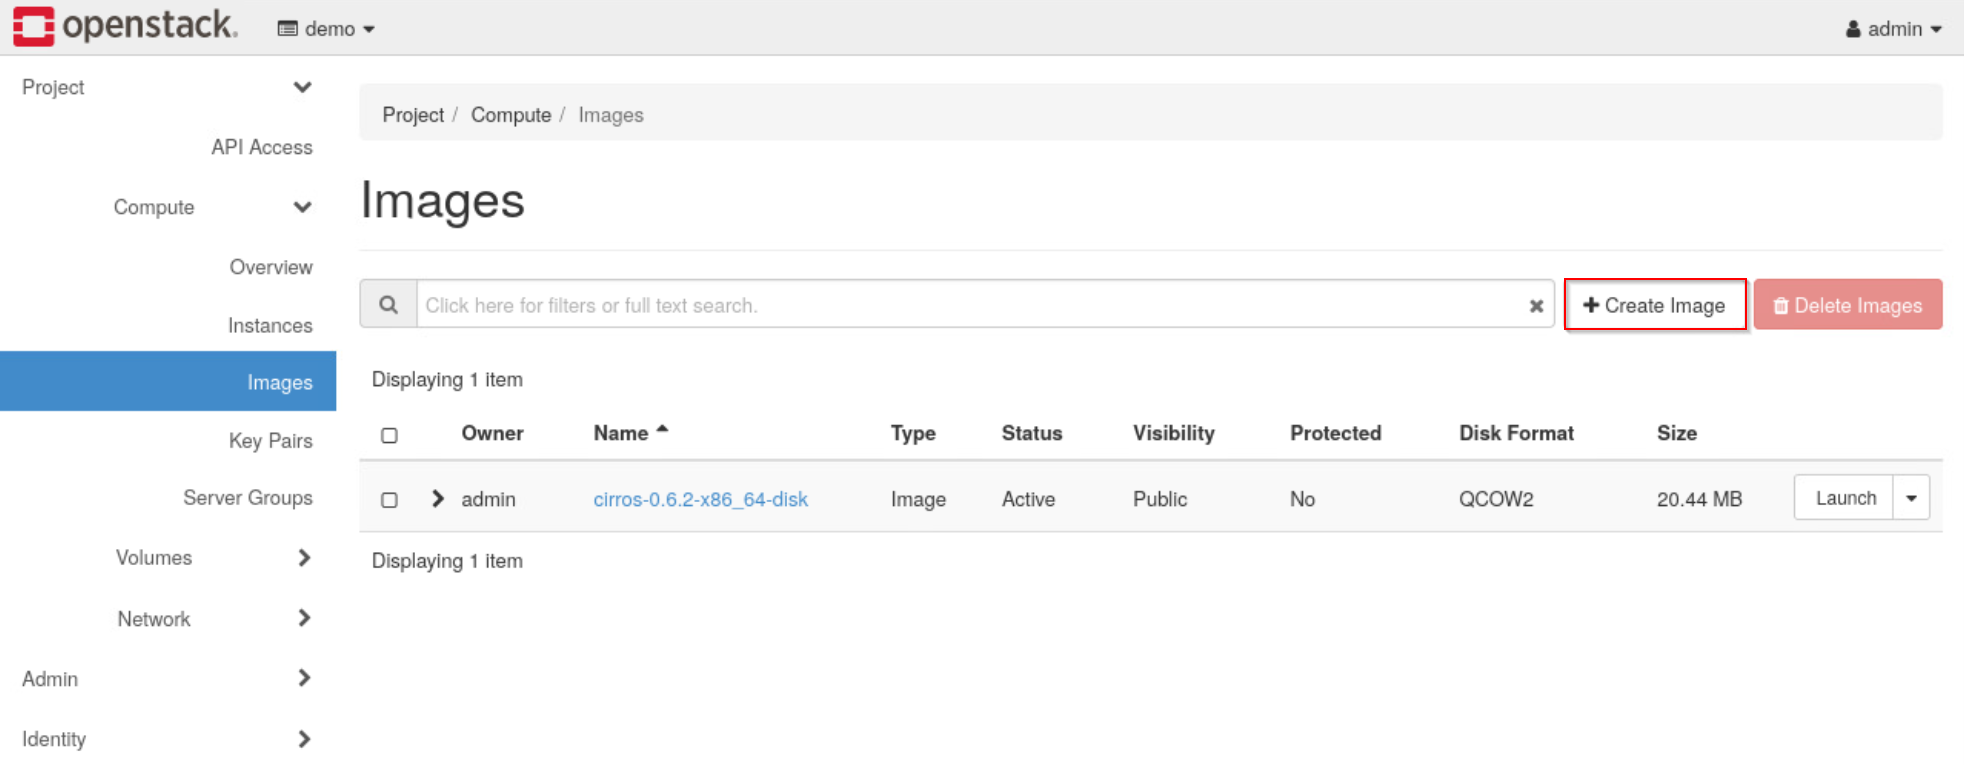
\includegraphics[width=\linewidth]{images/part1/step5.png}
    \end{center}

    \item Enter \textbf{ubuntu1} into the \textit{Image Name} field. Under \textbf{File}, click \textbf{Browse...}.
    
    \begin{center}
        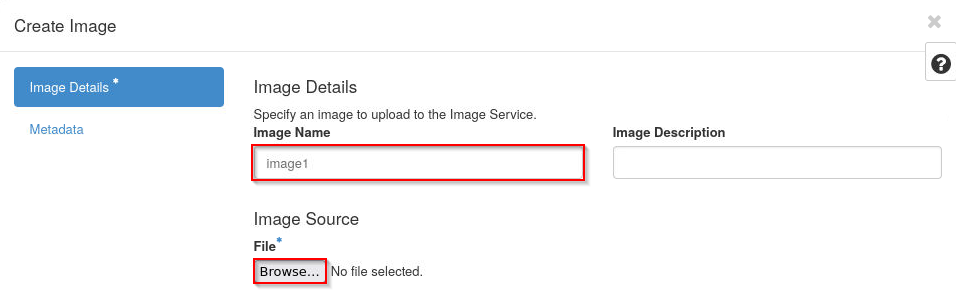
\includegraphics[width=\linewidth]{images/part1/step6.png}
    \end{center}

    \item In the file browser, click \textbf{Downloads}, then select the \textbf{ubuntu.img} file. Click the
    \textbf{Open} button.

    \begin{center}
        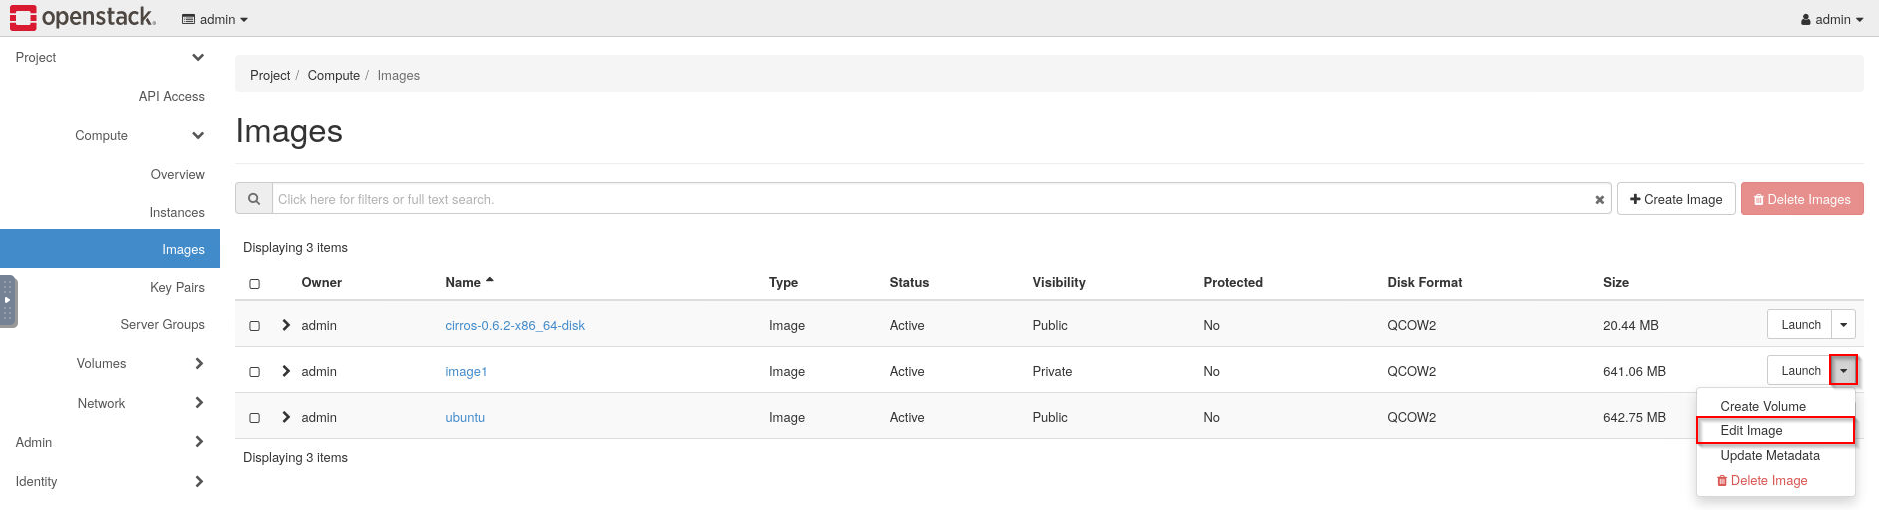
\includegraphics[width=\linewidth]{images/part1/step7.png}
    \end{center}

    \item In the format dropdown, select \textbf{QCOW2 - QEMU Emulator}, and under \textit{Image Sharing}, set
    \textit{Visibility} to \textbf{Private}. Make sure \textbf{No} is selected for \textit{Protected}, and click on
    \textbf{Create Image}.

    \begin{center}
        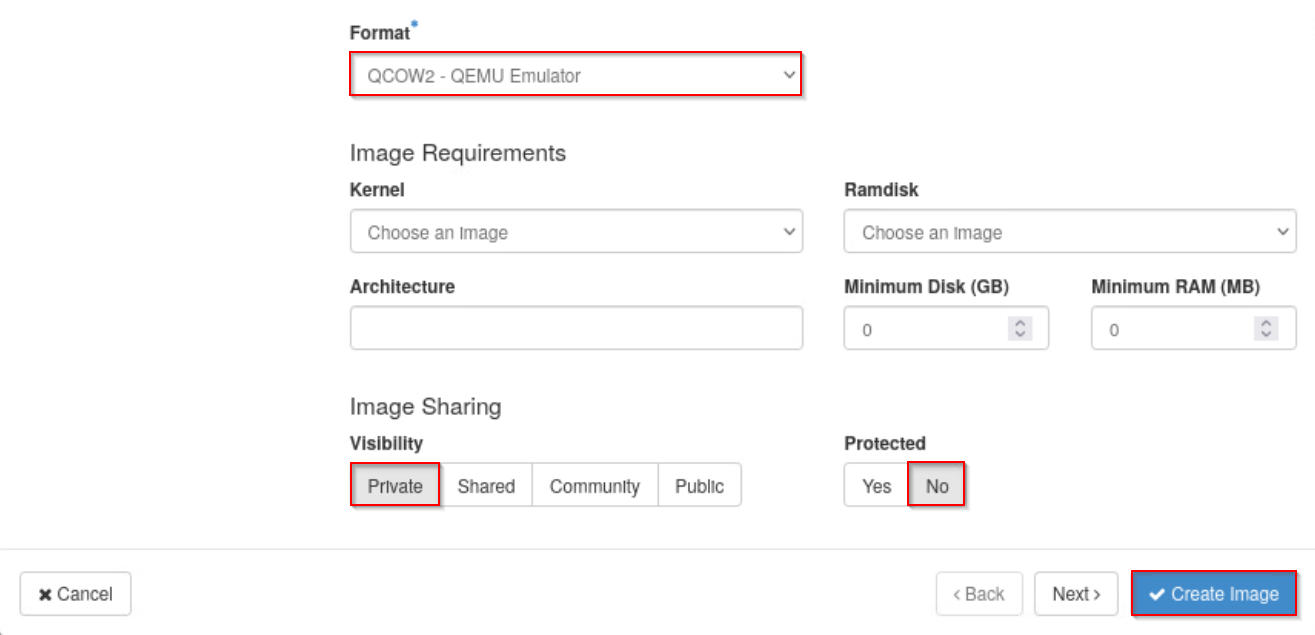
\includegraphics[width=\linewidth]{images/part1/step8.png}
    \end{center}

    \begin{stopbox}
        Wait for the \textbf{ubuntu1} status to be \textit{Active}. You may need to refresh the browser until you see the
        status of \textit{Active}.
    \end{stopbox}

    \item To edit the image after it has been created, open the dropdown menu next to the \textbf{Launch} button in the
    row of \textbf{ubuntu1}, and click on \textbf{Edit Image}.

    \begin{center}
        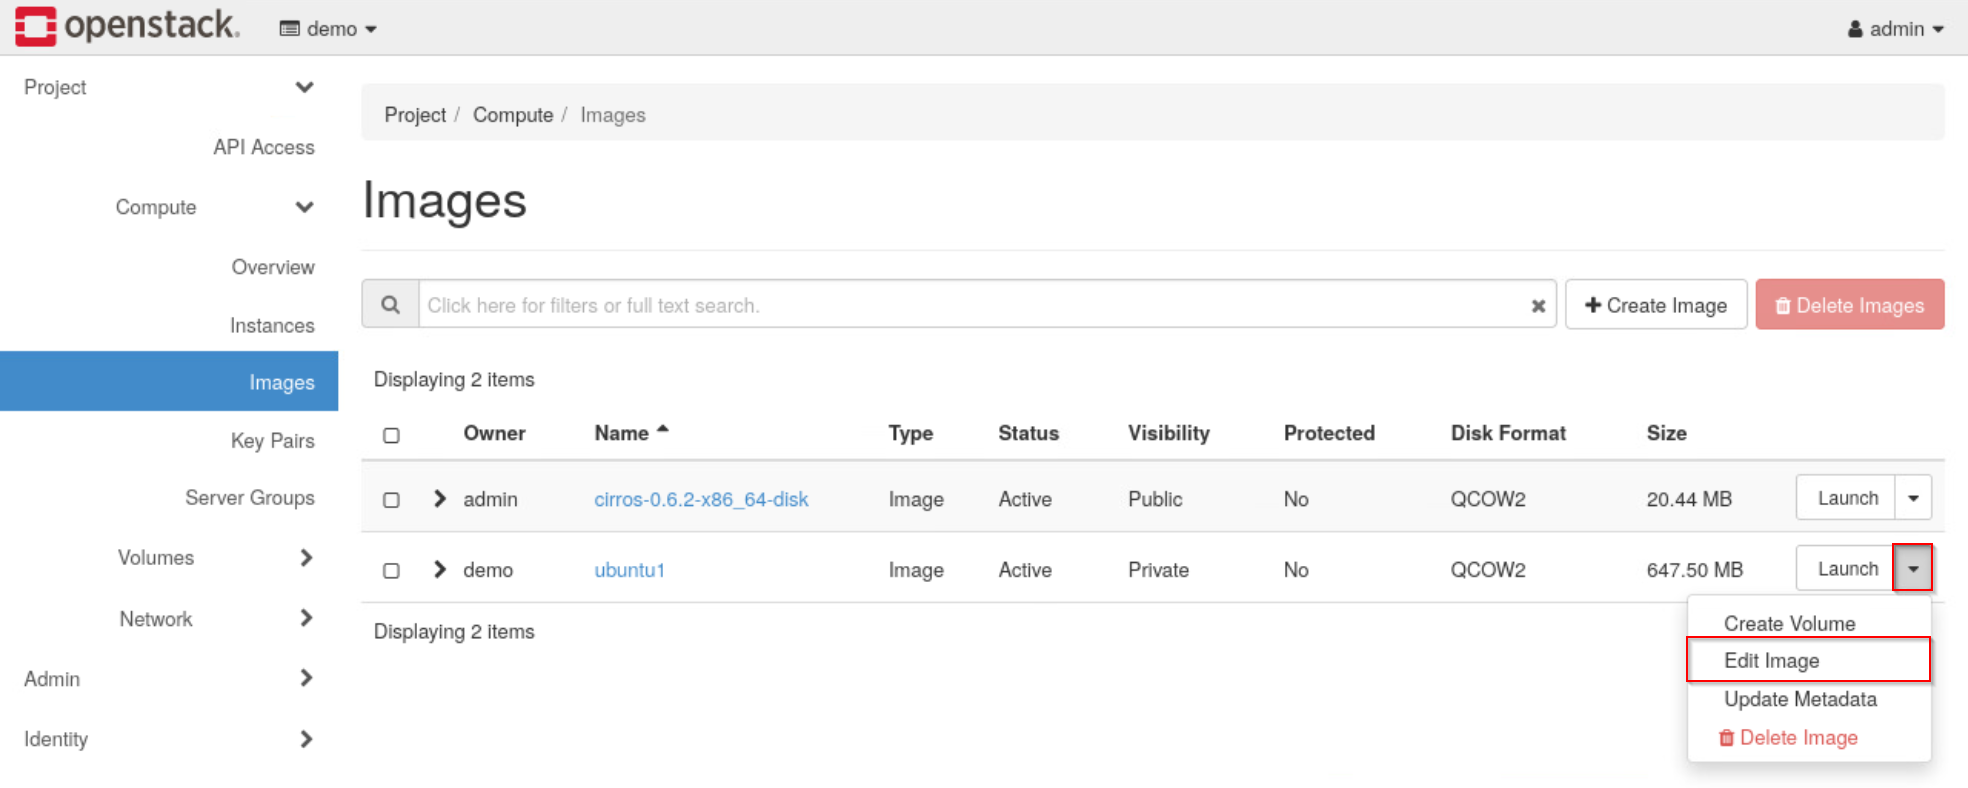
\includegraphics[width=\linewidth]{images/part1/step9.png}
    \end{center}

    \item Enter \textbf{10} in the \textit{Minimum Disk (GB)} field, and select \textbf{Yes} for \textit{Protected}.
    Click the \textbf{Update Image} button. Adding a minimum disk amount will require any new instance created with this
    image to allocate at least 10 GB of disk space. When an image or other OpenStack resource is protected, it cannot be
    deleted without first making it unprotected again.

    \begin{center}
        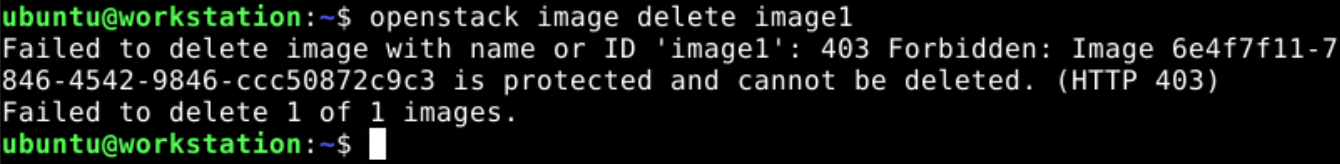
\includegraphics[width=\linewidth]{images/part1/step10.png}
    \end{center}

    \item Reopen the dropdown next to the \textbf{Launch} button in the same row as \textbf{ubuntu1}. Notice that the
    option to delete the image no longer appears because the image is protected.

    \begin{center}
        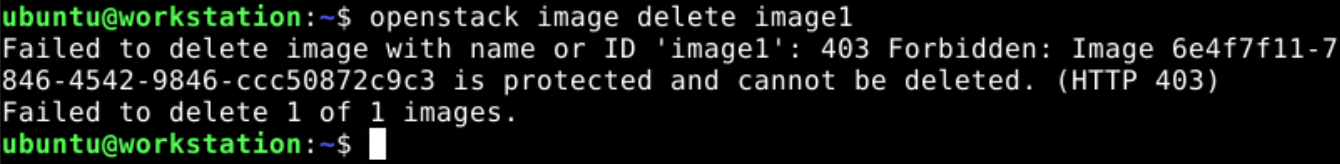
\includegraphics[width=\linewidth]{images/part1/step11.png}
    \end{center}

    \item Log out of the \textit{Horizon Dashboard} and close the web browser.

    \item Open a terminal if one is not already open, and source the \textbf{keystonerc-admin} file to load the
    \textbf{admin} user credentials.
    \begin{lstlisting}
        ubuntu@workstation:~$ source ~/keystonerc-admin
    \end{lstlisting}

    \begin{center}
        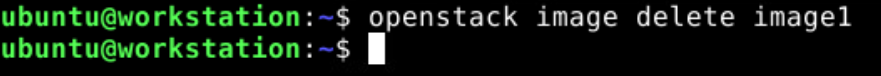
\includegraphics[width=\linewidth]{images/part1/step13.png}
    \end{center}

    \item List the current OpenStack images.
    \begin{lstlisting}
        [ubuntu@workstation (keystone-admin)]:~$ openstack image list
    \end{lstlisting}

    \begin{center}
        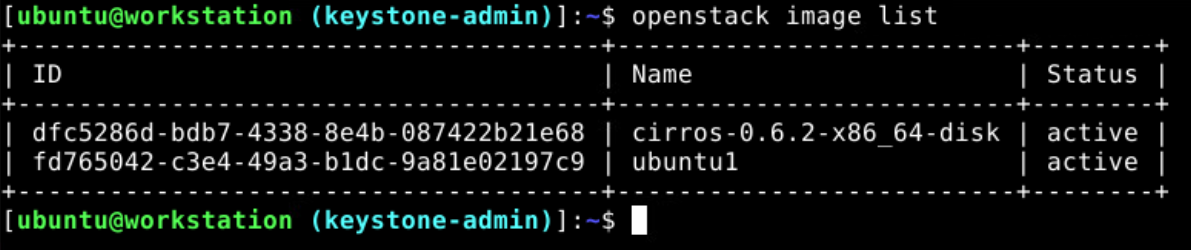
\includegraphics[width=\linewidth]{images/part1/step14.png}
    \end{center}

    \item Try to delete the \textbf{ubuntu1} image while it is protected. It should return an error.
    \begin{lstlisting}
        [ubuntu@workstation (keystone-admin)]:~$ openstack image delete ubuntu1
    \end{lstlisting}

    \begin{center}
        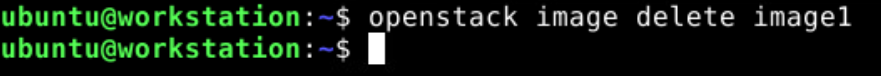
\includegraphics[width=\linewidth]{images/part1/step15.png}
    \end{center}

    \item Set the \textbf{ubuntu1} image to unprotected.
    \begin{lstlisting}
        [ubuntu@workstation (keystone-admin)]:~$ openstack image set \
        > --unprotected ubuntu1
    \end{lstlisting}

    \begin{center}
        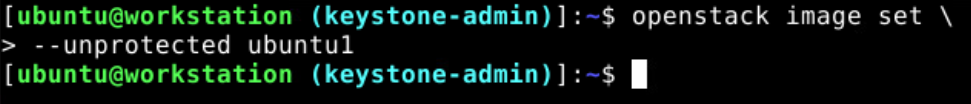
\includegraphics[width=\linewidth]{images/part1/step16.png}
    \end{center}

    \item Delete the \textbf{ubuntu1} image.
    \begin{lstlisting}
        [ubuntu@workstation (keystone-admin)]:~$ openstack image delete ubuntu1
    \end{lstlisting}

    \begin{center}
        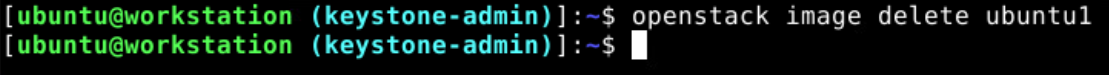
\includegraphics[width=\linewidth]{images/part1/step17.png}
    \end{center}

    \item List the images again to confirm that the image was deleted.
    \begin{lstlisting}
        [ubuntu@workstation (keystone-admin)]:~$ openstack image list
    \end{lstlisting}

    \begin{center}
        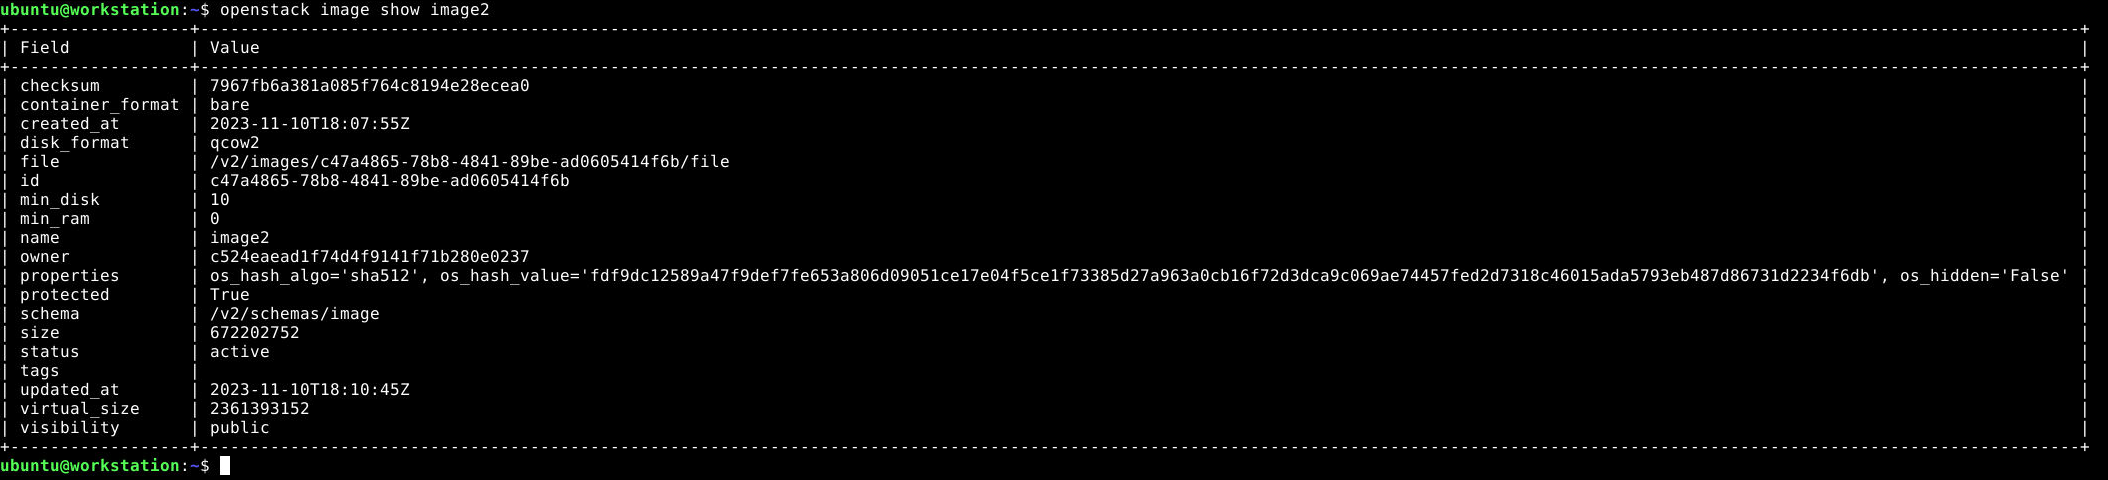
\includegraphics[width=\linewidth]{images/part1/step18.png}
    \end{center}

    \item Create the \textbf{ubuntu1} image using the \textbf{\texttildemid/Downloads/ubuntu.img} file and the QCOW2
    format.
    \begin{lstlisting}
        [ubuntu@workstation (keystone-admin)]:~$ openstack image create \
        > --disk-format qcow2 \
        > --file ~/Downloads/ubuntu.img \
        > ubuntu2
    \end{lstlisting}

    \begin{center}
        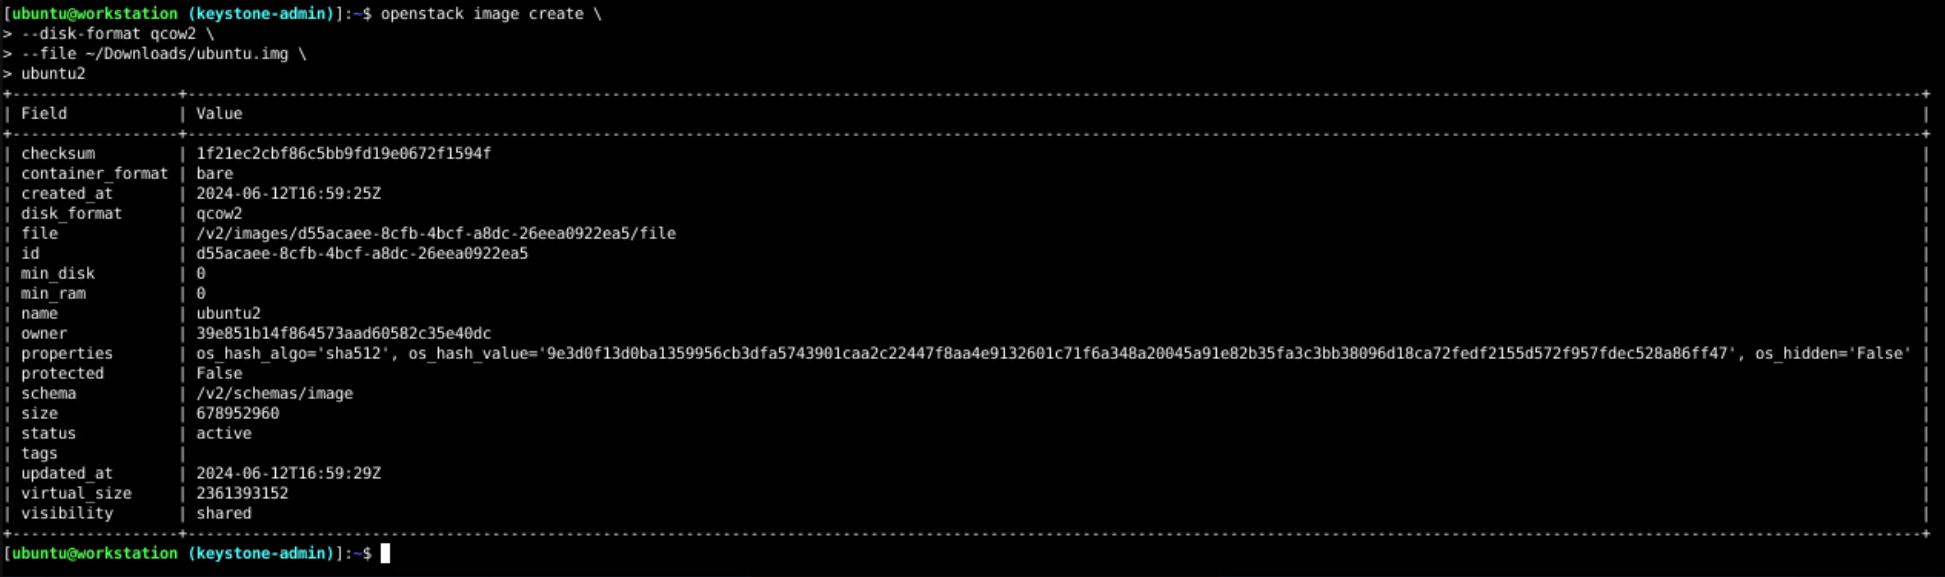
\includegraphics[width=\linewidth]{images/part1/step19.png}
    \end{center}

    \item Confirm that the image was created by listing the images again.
    \begin{lstlisting}
        [ubuntu@workstation (keystone-admin)]:~$ openstack image list
    \end{lstlisting}

    \item Set the \textbf{ubuntu2} image status to \textbf{protected}, and set the minimum disk size to \textbf{10 GB}.
    \begin{lstlisting}
        [ubuntu@workstation (keystone-admin)]:~$ openstack image set \
        > --protected \
        > --min-disk 10 \
        > ubuntu2
    \end{lstlisting}

    \begin{center}
        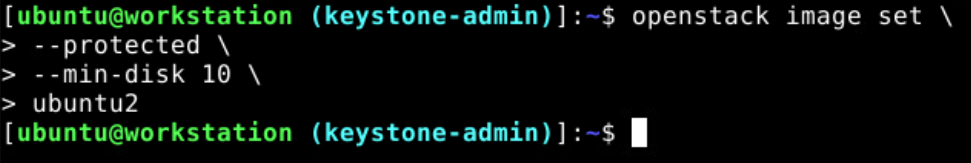
\includegraphics[width=\linewidth]{images/part1/step21.png}
    \end{center}

    \item If no visibility is set on creation, an image defaults to being private, which means the image is only visible
    to the user who created it. Set the \textbf{ubuntu2} image to be public so it is visible to other users. Note that
    this action requires administrative privileges.
    \begin{lstlisting}
        [ubuntu@workstation (keystone-admin)]:~$ openstack image set --public ubuntu2
    \end{lstlisting}

    \begin{center}
        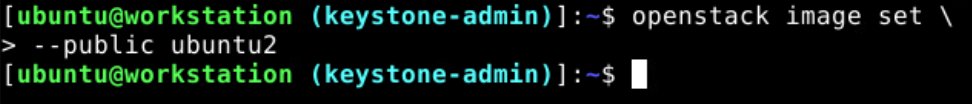
\includegraphics[width=\linewidth]{images/part1/step22.png}
    \end{center}

    \item Display the details of the \textbf{ubuntu2} image and verify that it was correctly updated. Confirm the value
    for the \textit{min\_disk} field is \textbf{10}, the value for the \textit{protected} field is \textbf{True}, and
    the value for \textit{visibility} is \textbf{public}.
    \begin{lstlisting}
        [ubuntu@workstation (keystone-admin)]:~$ openstack image show ubuntu2
    \end{lstlisting}

    \begin{center}
        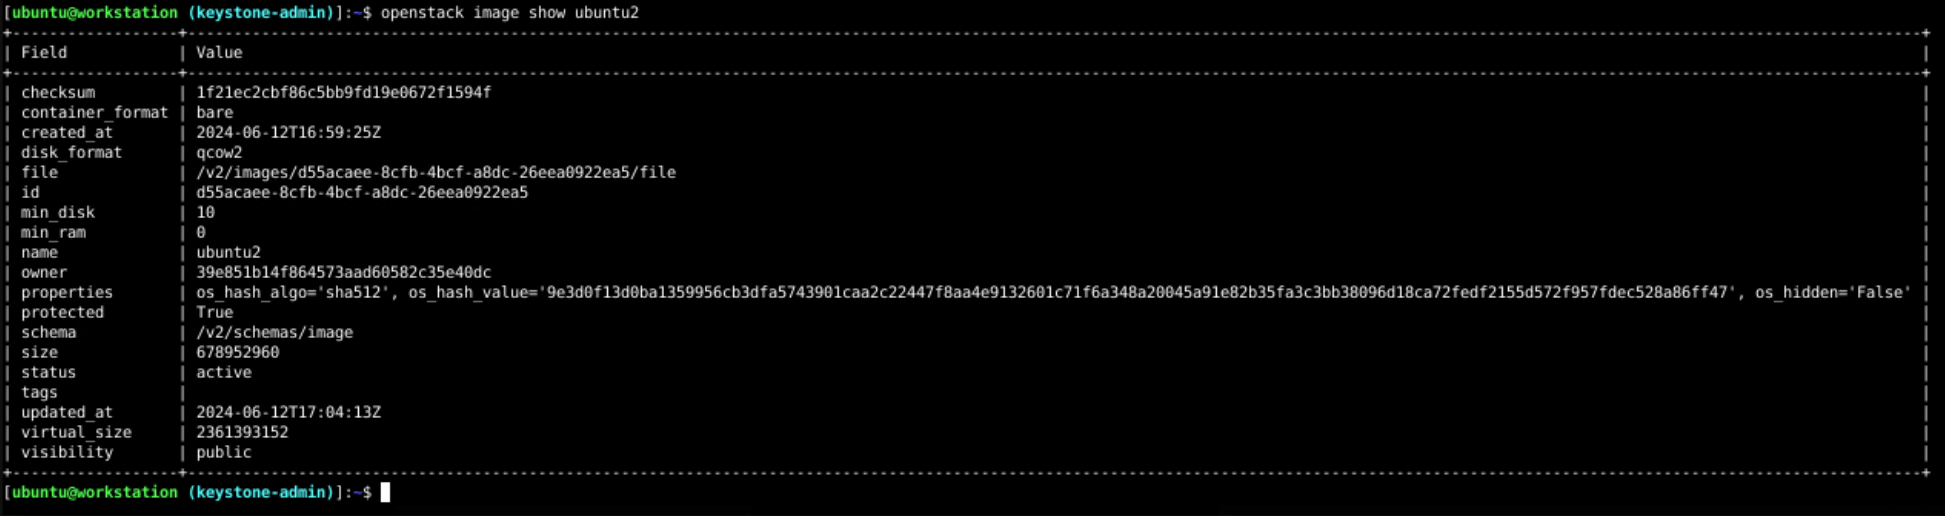
\includegraphics[width=\linewidth]{images/part1/step23.png}
    \end{center}

    \item Leave the terminal window open and continue to the next task.

\end{enumerate}

%%%%%%%%%%%
% Section 2
%%%%%%%%%%%
\section{Developing Flavors}
\label{sec:developing_flavors}
In this task, you will create and delete flavors using the \textit{Horizon Dashboard} and
\textit{OpenStack Unified CLI}.

\begin{enumerate}
    \item Open the web browser and navigate to \textbf{192.168.1.20}. Log in to the dashboard as the \textbf{admin} user
    with the password \textbf{secret}.
    
    \item Switch to the \textbf{demo} project. We will not need any of the existing flavors in this lab, and they can be
    safely deleted. For demonstration, navigate to \textbf{Admin $>$ Compute $>$ Flavors}, select the \textbf{ds1G}
    flavor, and click \textbf{Delete Flavors}.

    \begin{center}
        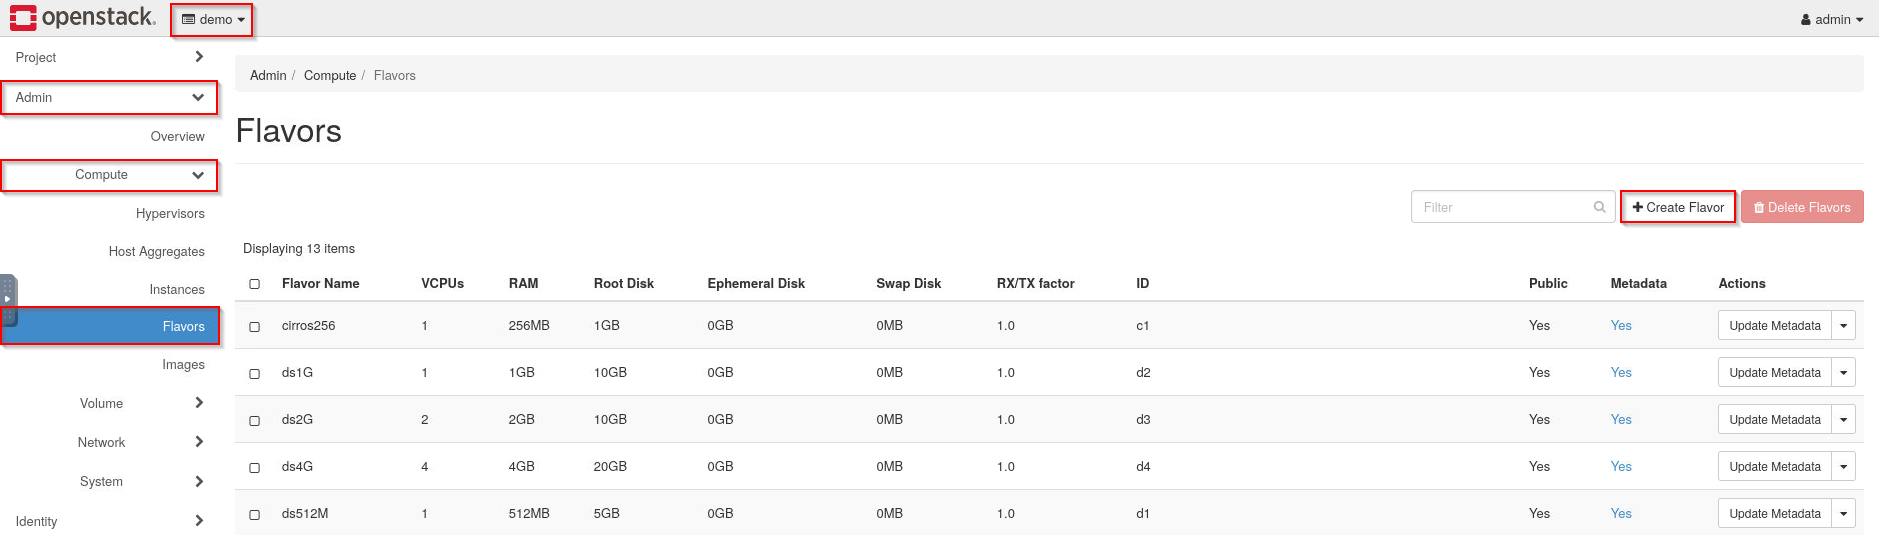
\includegraphics[width=\linewidth]{images/part2/step2.png}
    \end{center}

    \begin{tipbox}
        Alternatively, to delete a flavor, you can open the dropdown next to the \textbf{Update Metadata} button in the
        same row as the flavor, then click \textbf{Delete Flavor}.
    \end{tipbox}

    \item Now, we will create our own flavor. On the same page, click \textbf{Create Flavor}.

    \begin{center}
        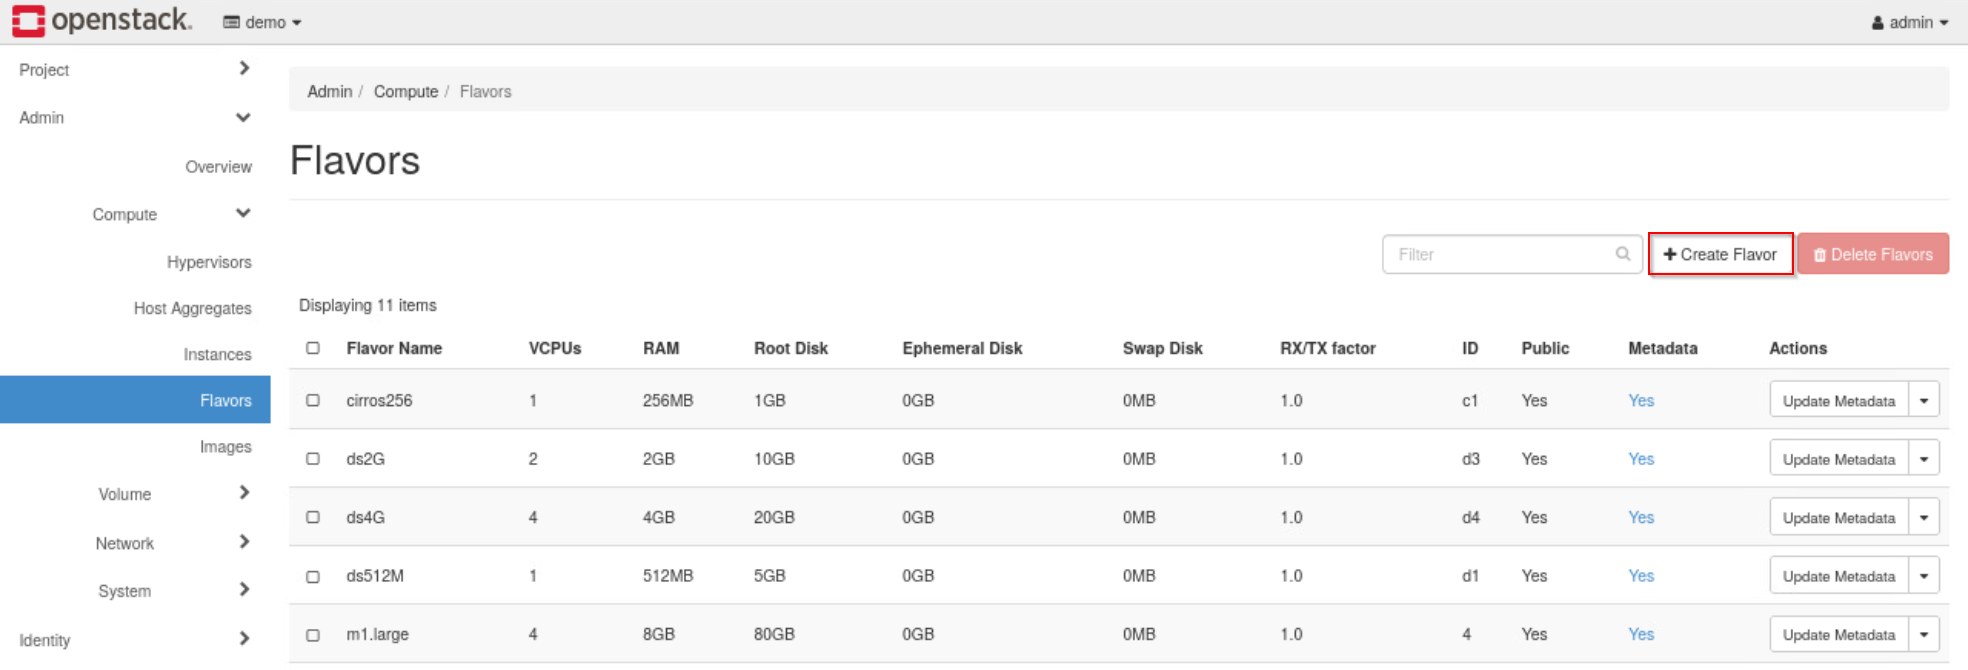
\includegraphics[width=\linewidth]{images/part2/step3.png}
    \end{center}

    \item Enter \textbf{flavor1} in the \textit{Name} field, \textbf{2} in the \textit{VCPUs} field, \textbf{1024} in
    the \textit{RAM (MB)} field, and \textbf{10} in the \textit{Root Disk (GB)} field. Click on \textbf{Create Flavor}.

    \begin{center}
        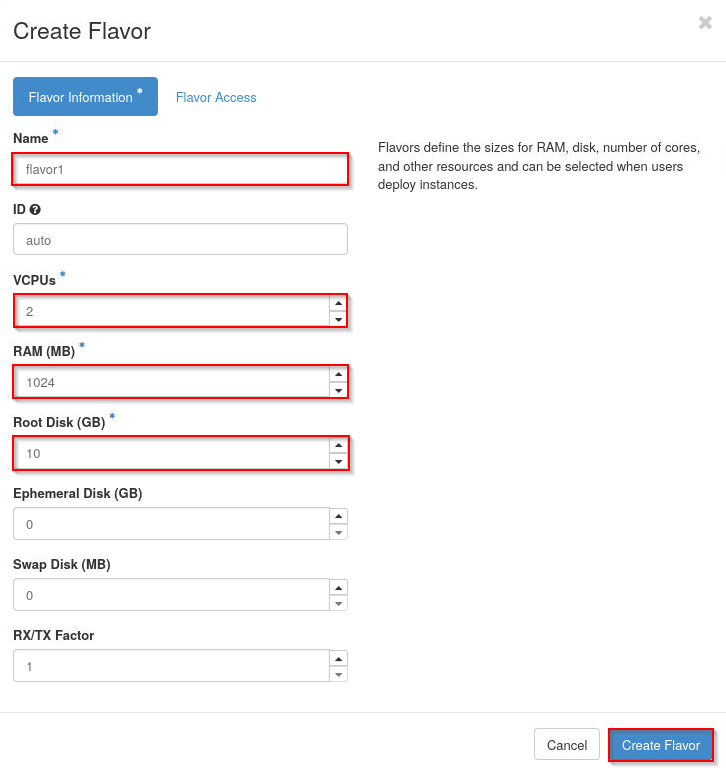
\includegraphics[width=\linewidth]{images/part2/step4.png}
    \end{center}

    \begin{notebox}
        There is currently no way to update flavors (apart from their metadata) from the Horizon Dashboard after a
        flavor has been created. Any changes will require deleting the flavor and remaking it.
    \end{notebox}

    \item Log out of the \textit{Horizon Dashboard} and close the web browser.
    
    \item If a terminal is not already open, open one and source the \textbf{\texttildemid/keystonerc-admin} file.
    \begin{lstlisting}
        ubuntu@workstation:~$ source ~/keystonerc-admin
    \end{lstlisting}

    \begin{center}
        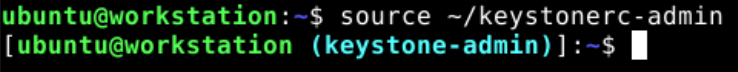
\includegraphics[width=\linewidth]{images/part2/step6.png}
    \end{center}

    \item List the current OpenStack flavors.
    \begin{lstlisting}
        [ubuntu@workstation (keystone-admin)]:~$ openstack flavor list
    \end{lstlisting}

    \begin{center}
        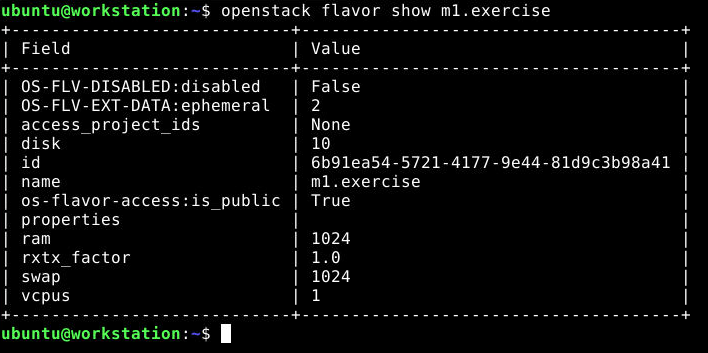
\includegraphics[width=\linewidth]{images/part2/step7.png}
    \end{center}

    \item Create a flavor named \textbf{flavor2}. Configure the flavor with \textbf{1} VCPU, \textbf{1024 MB} of RAM, a
    \textbf{10 GB} root disk, a \textbf{2 GB} ephemeral disk, and a \textbf{1024 MB} swap disk.
    \begin{lstlisting}
        [ubuntu@workstation (keystone-admin)]:~$ openstack flavor create \
        > --vcpus 1 \
        > --ram 1024 \
        > --disk 10 \
        > --ephemeral 2 \
        > --swap 1024 \
        > flavor2
    \end{lstlisting}

    \begin{center}
        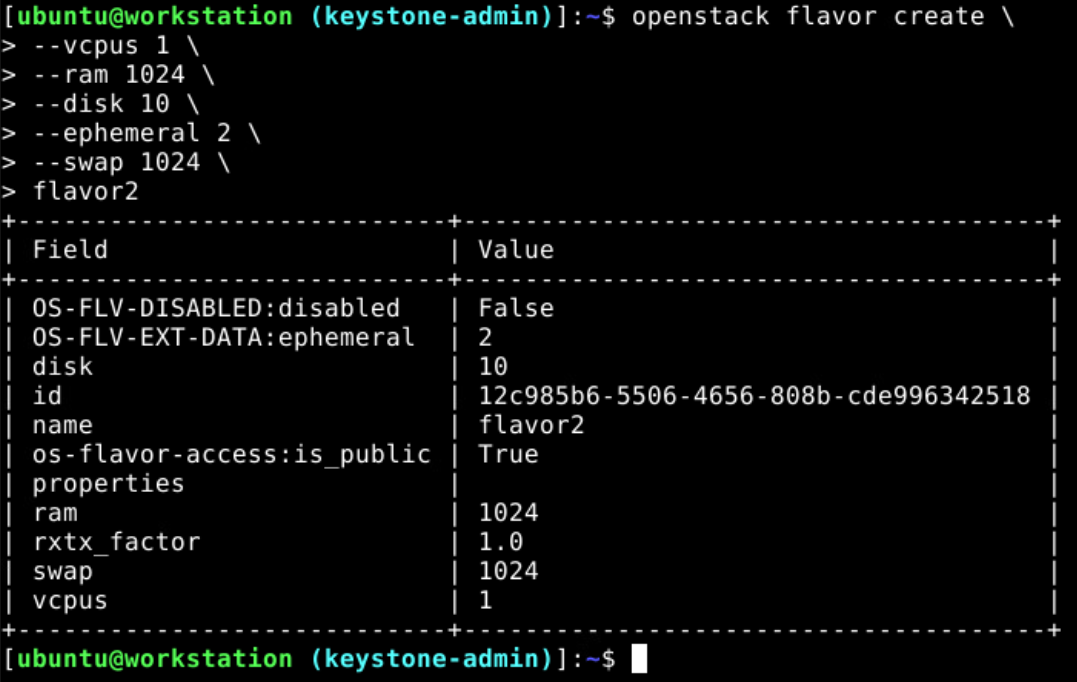
\includegraphics[width=\linewidth]{images/part2/step8.png}
    \end{center}

    \begin{notebox}
        Ephemeral storage is storage that, from the user's point of view, disappears when an instance is terminated.
        Swap space allows the operating system to use a portion of hard disk space as additional RAM if the physical
        memory becomes full.
    \end{notebox}

    \item Verify that the \textbf{flavor2} flavor has been created and has the correct values by listing the flavors.
    \begin{lstlisting}
        [ubuntu@workstation (keystone-admin)]:~$ openstack flavor list
    \end{lstlisting}

    \begin{center}
        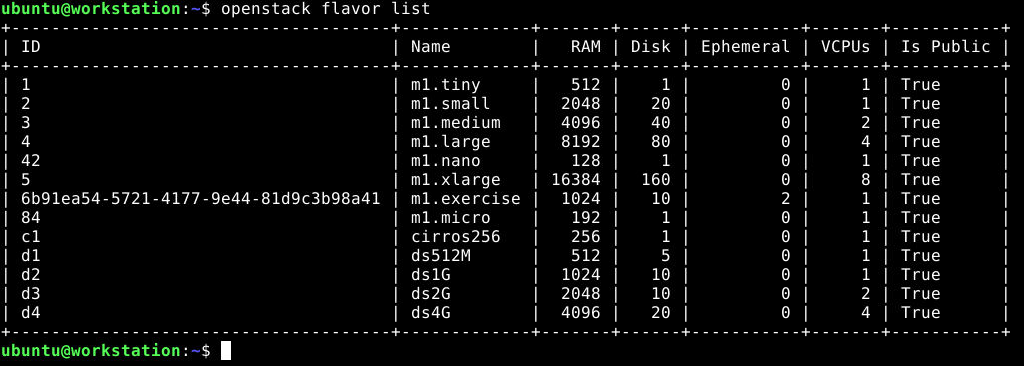
\includegraphics[width=\linewidth]{images/part2/step9.png}
    \end{center}

    \item Show more details about \textbf{flavor2}.
    \begin{lstlisting}
        [ubuntu@workstation (keystone-admin)]:~$ openstack flavor show flavor2
    \end{lstlisting}

    \begin{center}
        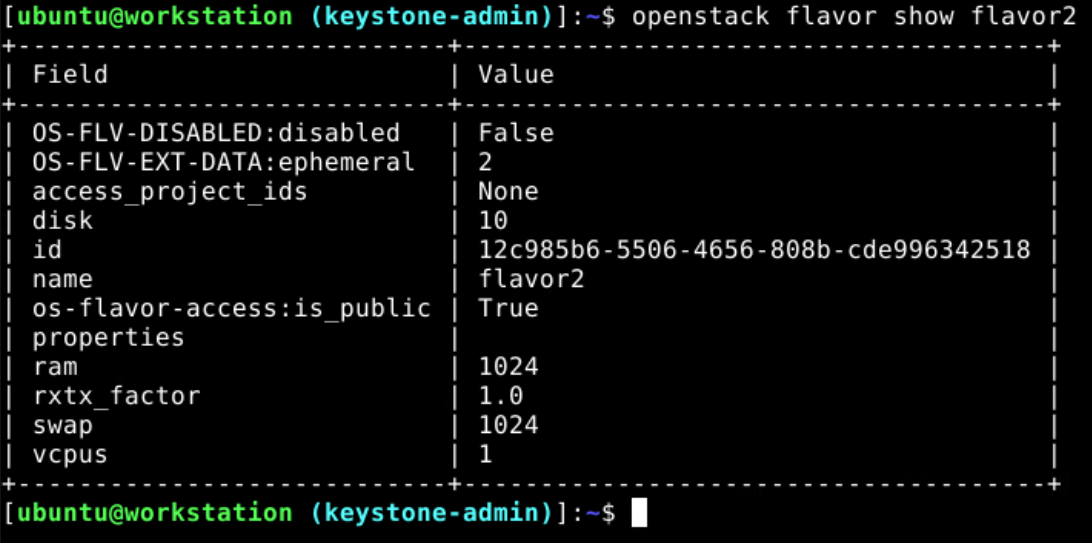
\includegraphics[width=\linewidth]{images/part2/step10.png}
    \end{center}

    \item The \textbf{flavor1} flavor is no longer needed. Delete the \textbf{flavor1} flavor to demonstrate deletion
    from the command line.
    \begin{lstlisting}
        [ubuntu@workstation (keystone-admin)]:~$ openstack flavor delete flavor1
    \end{lstlisting}

    \begin{center}
        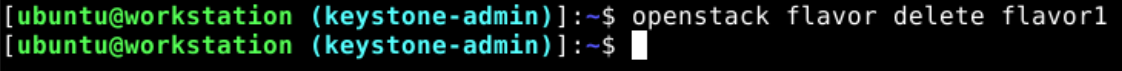
\includegraphics[width=\linewidth]{images/part2/step11.png}
    \end{center}

    \item Verify that the \textbf{flavor1} has been deleted by listing all the available flavors and noting that
    \textbf{flavor1} does not appear in the list.
    \begin{lstlisting}
        [ubuntu@workstation (keystone-admin)]:~$ openstack flavor list    
    \end{lstlisting}

    \begin{center}
        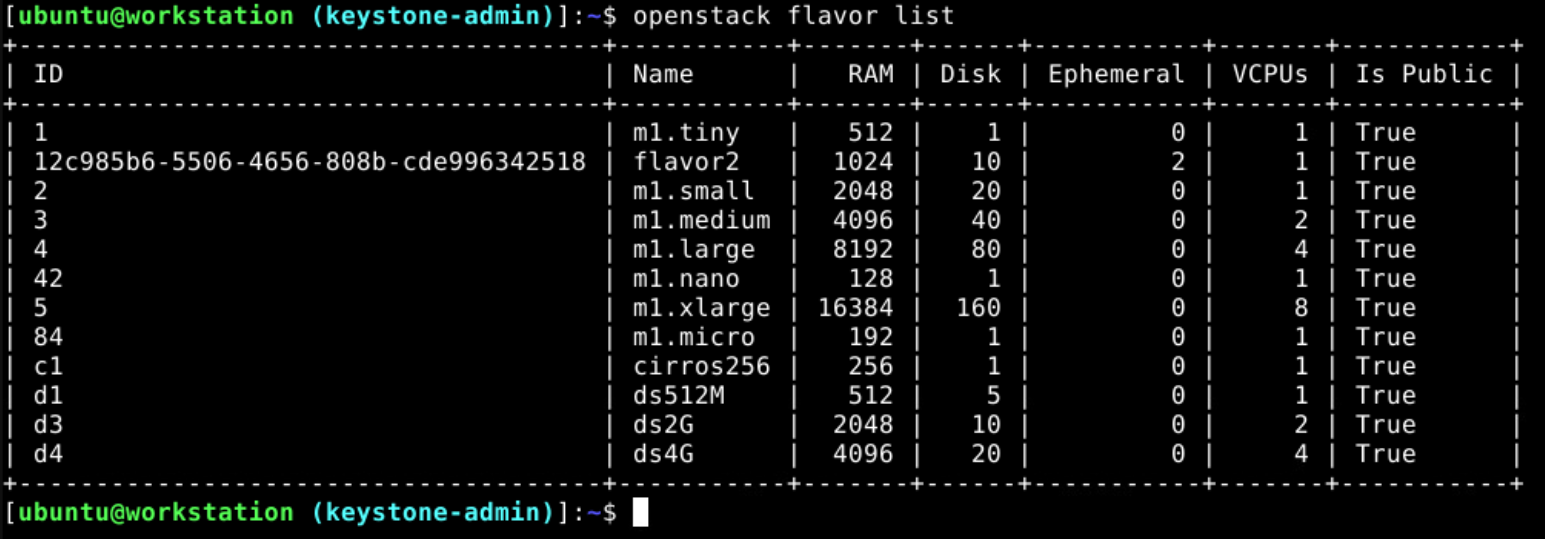
\includegraphics[width=\linewidth]{images/part2/step12.png}
    \end{center}

    \begin{tipbox}
        An alternative method is appending \textbf{\texttt{| grep flavor1}} to this command and noting that the output
        is empty.
    \end{tipbox}

    \begin{notebox}
        There are currently no standard OpenStack commands to update a flavor after creation. Any changes will require
        deleting the flavor and remaking it.
    \end{notebox}

    \item Leave the terminal window open and continue to the next task.
\end{enumerate}

%%%%%%%%%%%
% Section 3
%%%%%%%%%%%
\section{Managing Private Networks}
\label{sec:managing_private_networks}
In this task, you will manage networks and subnets using the \textit{Horizon Dashboard} and \textit{OpenStack
Unified CLI}. You will create and delete networks and subnetworks, update their settings, and rename them.

\begin{enumerate}
    \item Open the web browser and navigate to \textbf{192.168.1.20}. Log in to the dashboard as the \textbf{admin} user
    with the password \textbf{secret}.

    \item Switch to the \textbf{demo} project. We will create and manage our own networks in this lab, so any existing
    network can be safely deleted. To delete a network, all of its ports must first be deleted. Navigate to
    \textbf{Project $>$ Network $>$ Networks} and click on the \textbf{shared} network.

    \begin{center}
        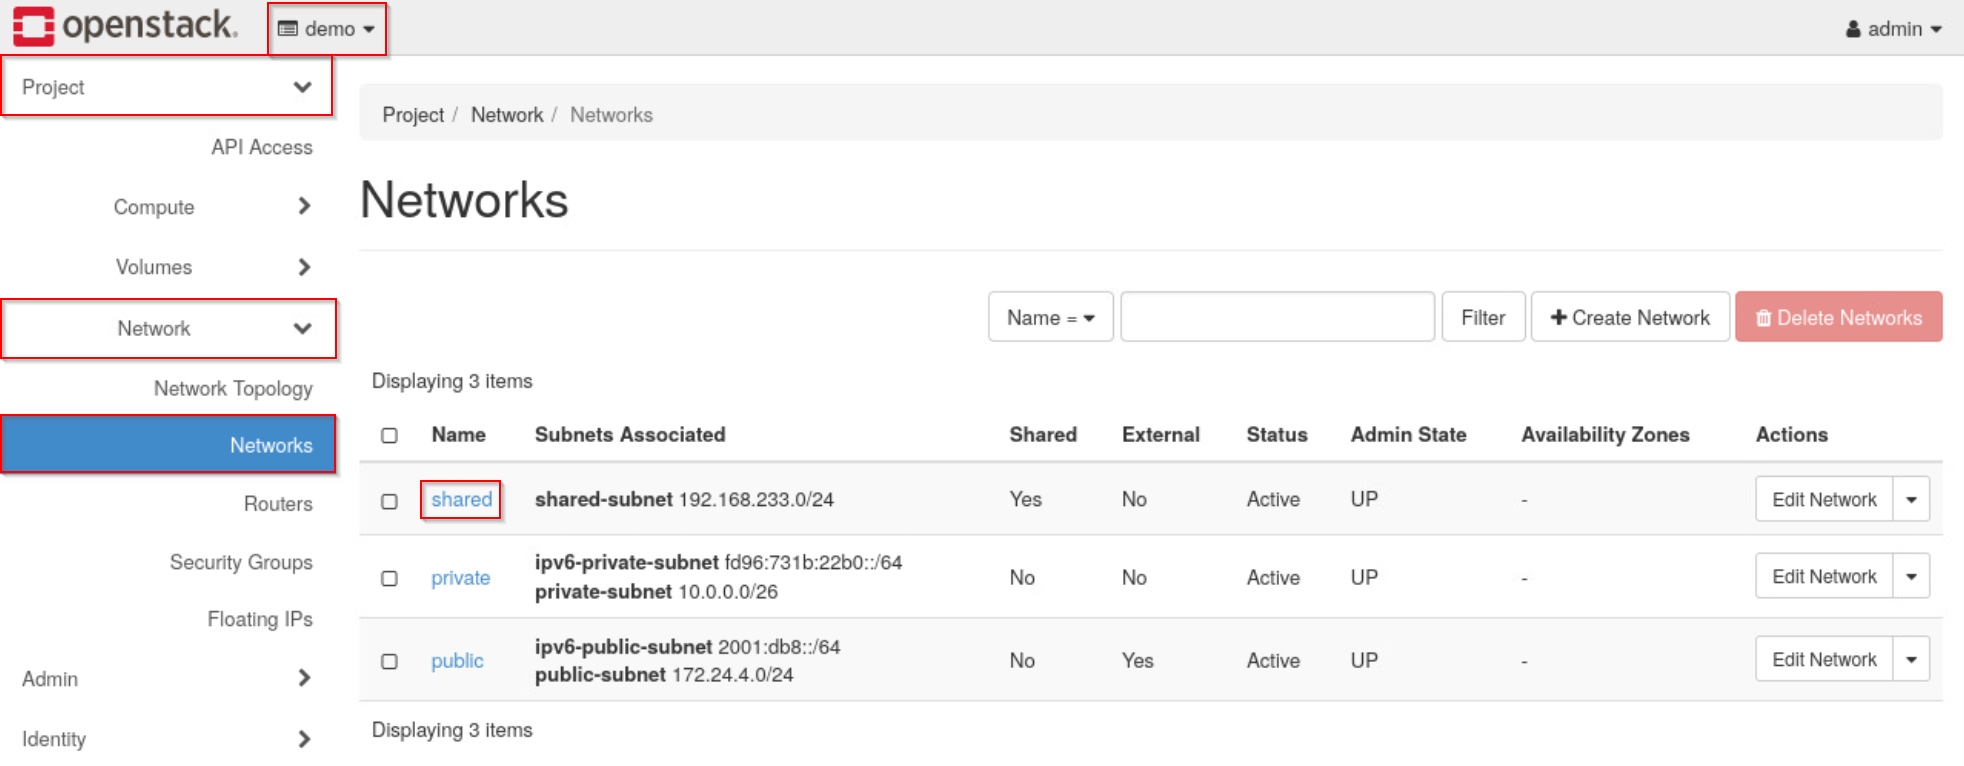
\includegraphics[width=\linewidth]{images/part3/step2.png}
    \end{center}

    \item Navigate to the \textbf{Ports} tab. Select all ports and click \textbf{Delete Ports}.

    \begin{center}
        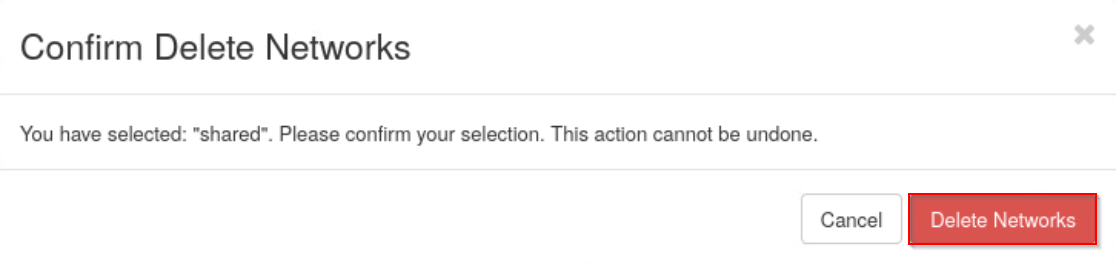
\includegraphics[width=\linewidth]{images/part3/step3.png}
    \end{center}

    \begin{tipbox}
        We will see in the next lab that if a network is attached to a router, the interfaces connecting the network to
        the router must be deleted from the router side, or the entire router could be deleted. Then, once all ports of
        the network have been deleted, the network itself can be deleted.
    \end{tipbox}

    \item Click \textbf{Delete Ports} in the popup box to confirm deletion.

    \begin{center}
        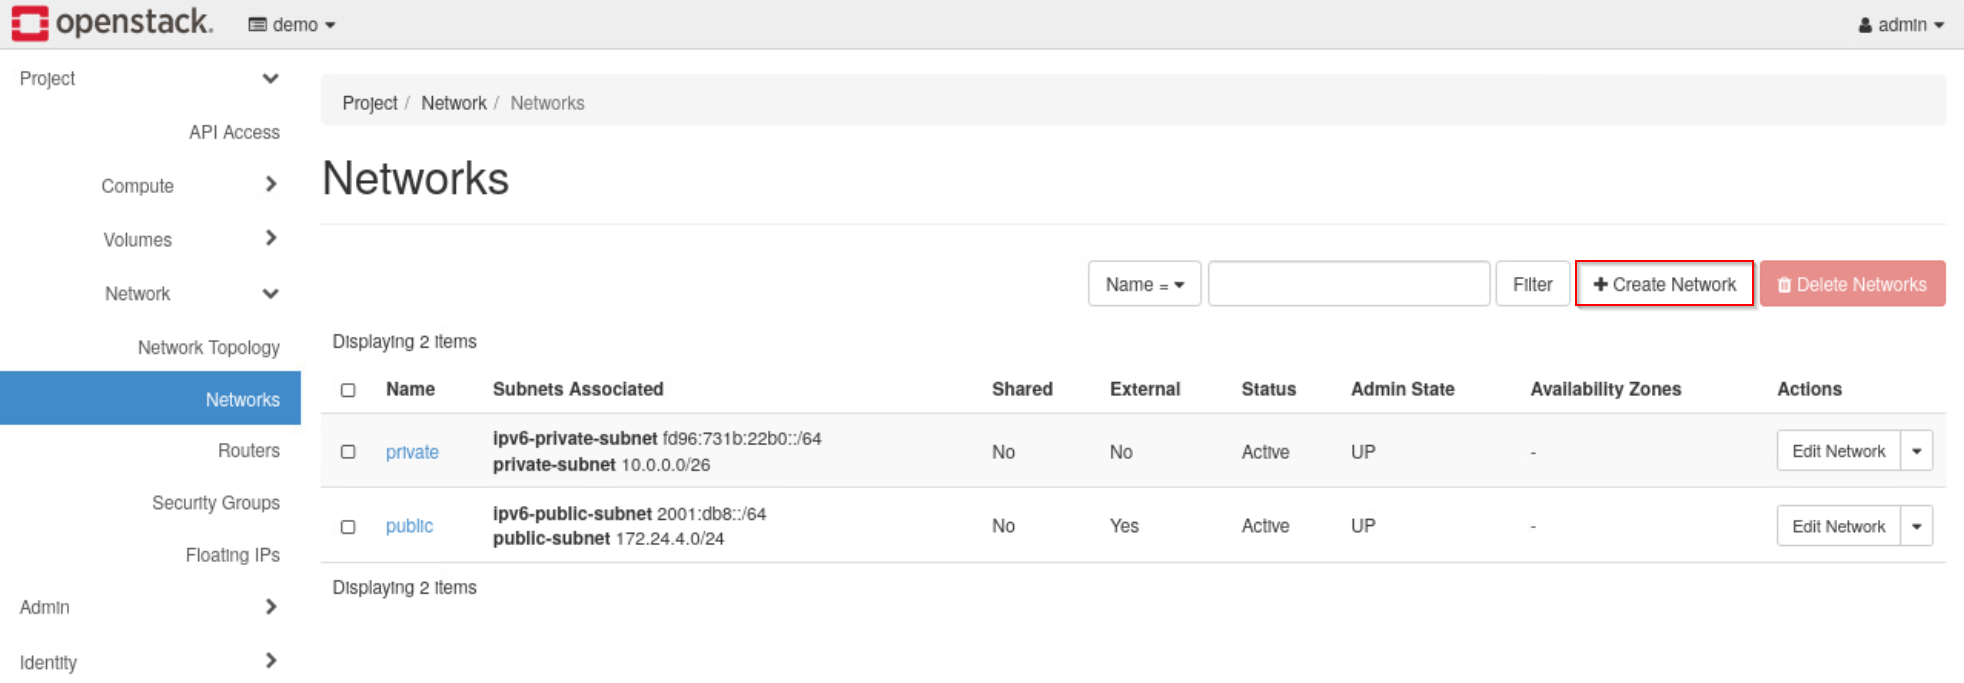
\includegraphics[width=\linewidth]{images/part3/step4.png}
    \end{center}

    \item Finally, to delete the \textbf{shared} network, navigate back to \textbf{Project $>$ Network $>$ Networks},
    select the \textbf{shared} network, and click \textbf{Delete Networks}.

    \begin{center}
        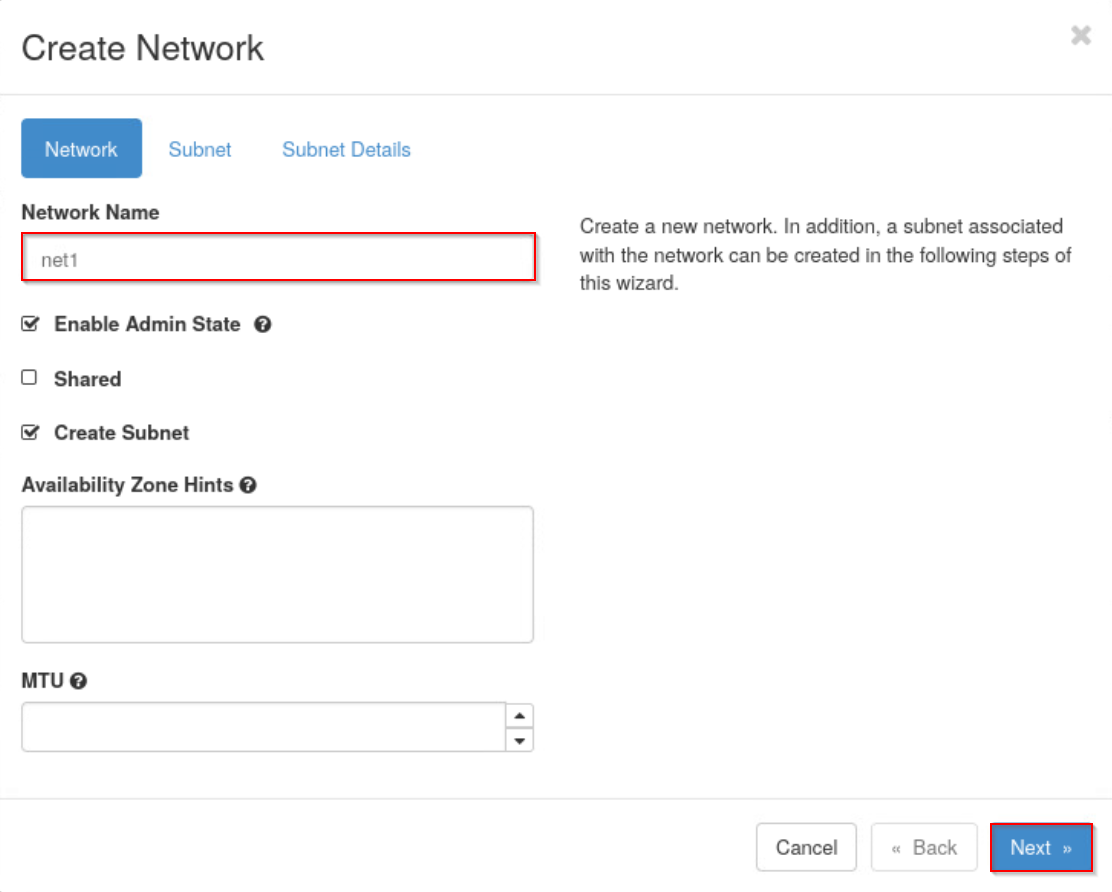
\includegraphics[width=\linewidth]{images/part3/step5.png}
    \end{center}

    \item Click \textbf{Delete Networks} in the popup box to confirm deletion.

    \begin{center}
        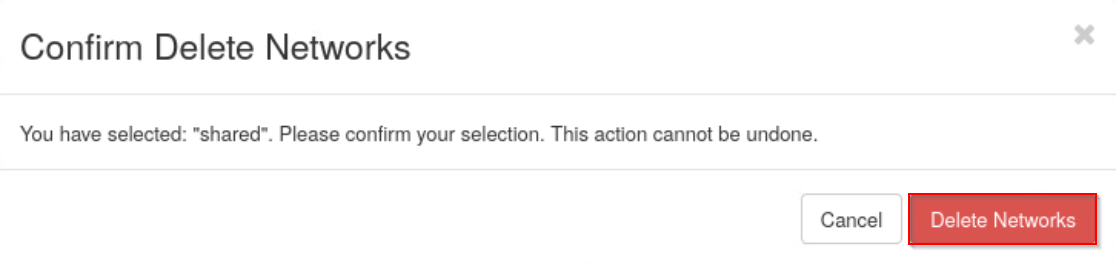
\includegraphics[width=\linewidth]{images/part3/step6.png}
    \end{center}

    \item Now, we will create our own network and subnet. Navigate back to \textbf{Project $>$ Network $>$ Networks} and
    click \textbf{Create Network}.

    \begin{center}
        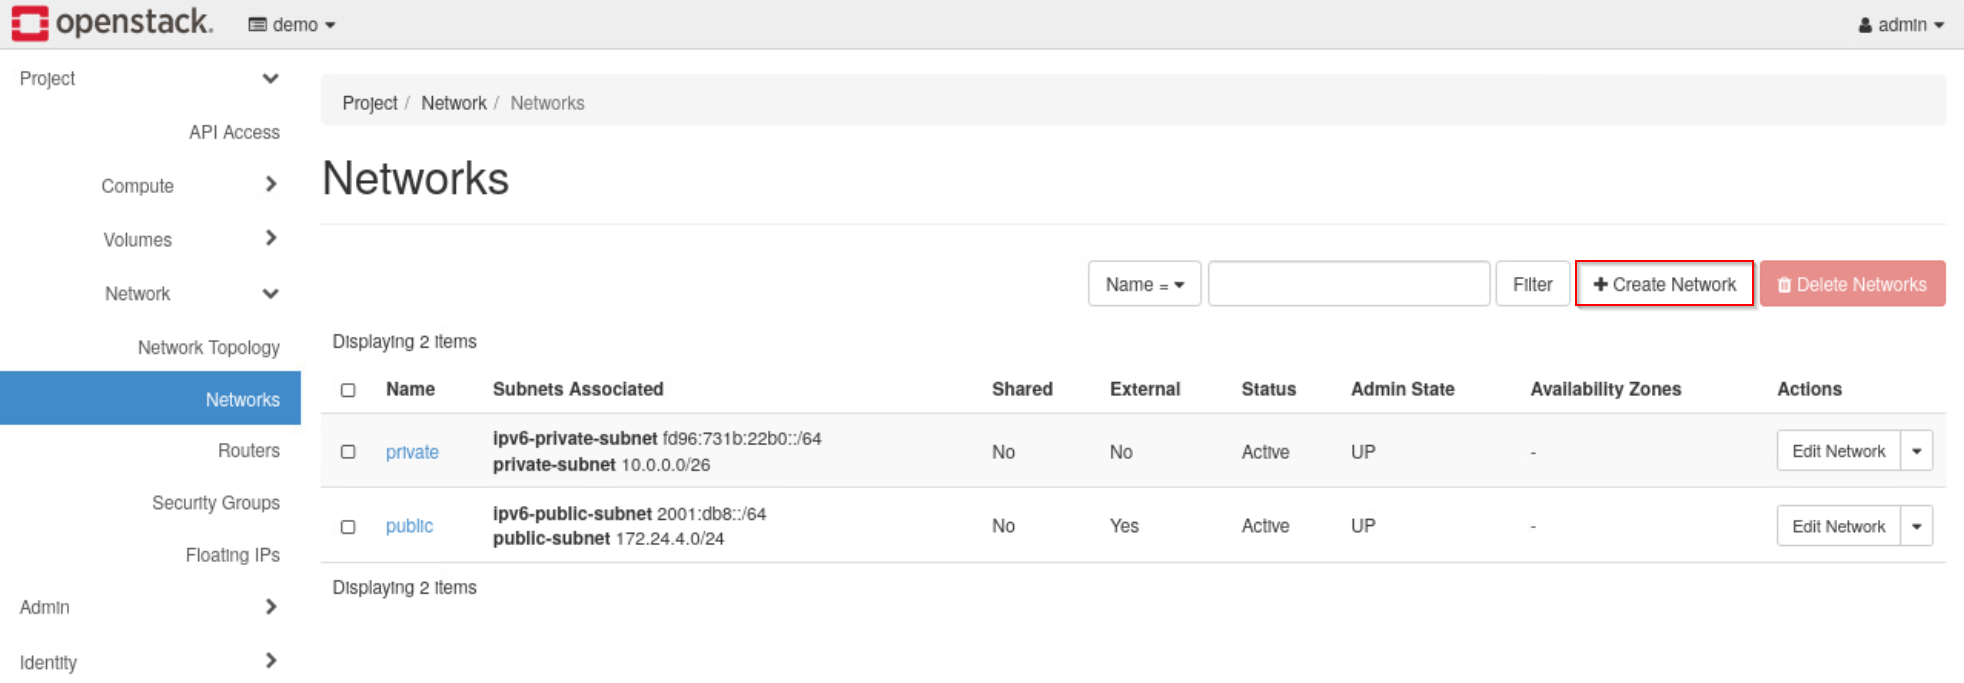
\includegraphics[width=\linewidth]{images/part3/step7.png}
    \end{center}

    \item Enter \textbf{net1} in the \textit{Network Name} field. Verify that the \textbf{Create Subnet} check box is
    selected. Click \textbf{Next}.

    \begin{center}
        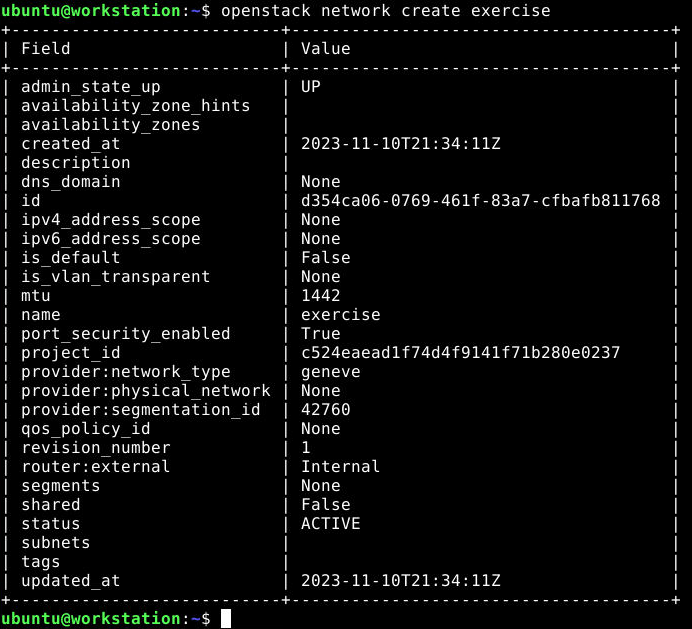
\includegraphics[width=\linewidth]{images/part3/step8.png}
    \end{center}

    \item Enter \textbf{subnet1} in the \textit{Subnet Name} field, and enter \textbf{10.0.0.0/24} in the
    \textit{Network Address} field. Click \textbf{Next}.

    \begin{center}
        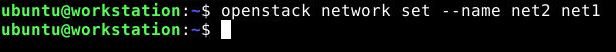
\includegraphics[width=\linewidth]{images/part3/step9.png}
    \end{center}

    \item Leave the defaults in the \textit{Subnet Details} tab and click \textbf{Create}.
    
    \begin{center}
        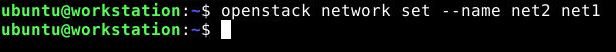
\includegraphics[width=\linewidth]{images/part3/step10.png}
    \end{center}

    \item Log out of the \textit{Horizon Dashboard} and close the web browser.
    
    \item If a terminal window is not already open, open one and source the \textbf{\texttildemid/keystonerc-admin} file
    to load the \textbf{admin} user credentials.
    \begin{lstlisting}
        ubuntu@workstation:~$ source ~/keystonerc-admin
    \end{lstlisting}

    \begin{center}
        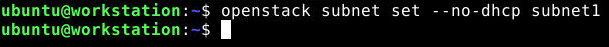
\includegraphics[width=\linewidth]{images/part3/step12.png}
    \end{center}

    \item List the current OpenStack networks.
    \begin{lstlisting}
        [ubuntu@workstation (keystone-admin)]:~$ openstack network list
    \end{lstlisting}

    \begin{center}
        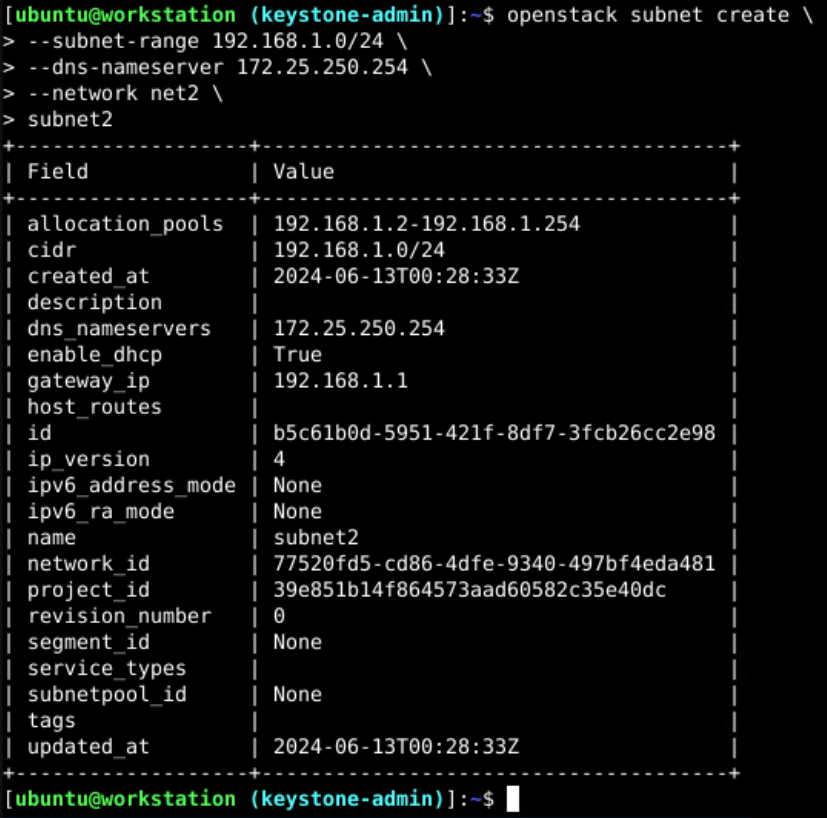
\includegraphics[width=\linewidth]{images/part3/step13.png}
    \end{center}

    \item Create a network named \textbf{net2} using the command below.
    \begin{lstlisting}
        [ubuntu@workstation (keystone-admin)]:~$ openstack network create net2
    \end{lstlisting}

    \begin{center}
        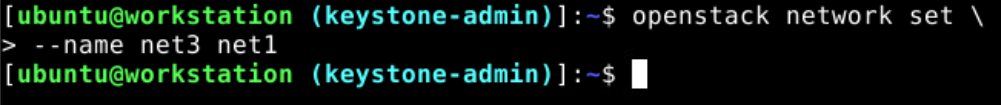
\includegraphics[width=\linewidth]{images/part3/step14.png}
    \end{center}

    \item List the networks again to confirm that the network was successfully created.
    \begin{lstlisting}
        [ubuntu@workstation (keystone-admin)]:~$ openstack network list
    \end{lstlisting}

    \begin{center}
        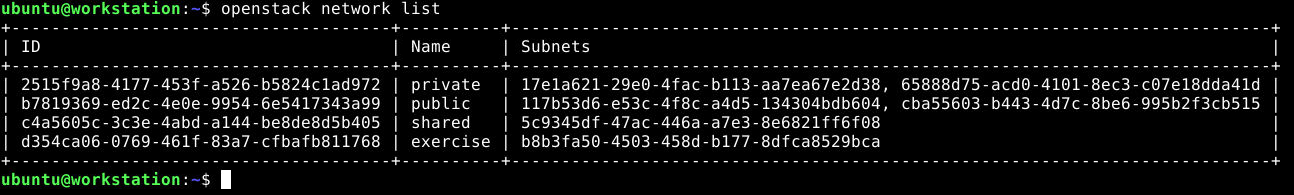
\includegraphics[width=\linewidth]{images/part3/step15.png}
    \end{center}

    \item Create a subnet named \textbf{subnet2} for the \textbf{net2} network. Configure this subnet to use the
    \textbf{192.168.1.0./24} range and \textbf{172.25.250.254} as the DNS name server.
    \begin{lstlisting}
        [ubuntu@workstation (keystone-admin)]:~$ openstack subnet create \
        > --subnet-range 192.168.1.0/24 \
        > --dns-nameserver 172.25.250.254 \
        > --network net2 \
        > subnet2
    \end{lstlisting}

    \begin{center}
        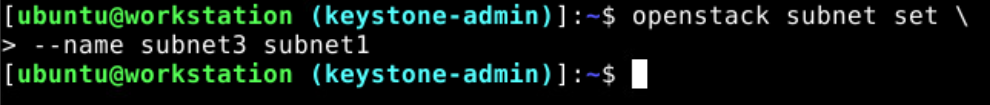
\includegraphics[width=\linewidth]{images/part3/step16.png}
    \end{center}

    \item The name of a network can also be changed. To demonstrate this, change the name of the \textbf{net1} network
    to \textbf{net3}.
    \begin{lstlisting}
        [ubuntu@workstation (keystone-admin)]:~$ openstack network set \
        > --name net3 net1
    \end{lstlisting}

    \begin{center}
        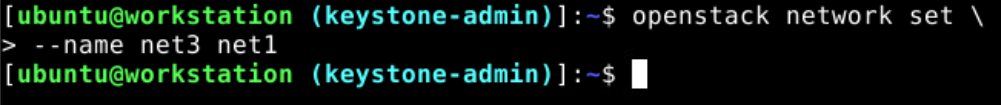
\includegraphics[width=\linewidth]{images/part3/step17.png}
    \end{center}

    \begin{notebox}
        The desired name for the network follows the \textbf{\texttt{--name}} option, while the current network name is
        the final argument of the command.
    \end{notebox}

    \item Verify that the \textbf{net1} network has been successfully changed to \textbf{net3}.
    \begin{lstlisting}
        [ubuntu@workstation (keystone-admin)]:~$ openstack network list
    \end{lstlisting}

    \begin{center}
        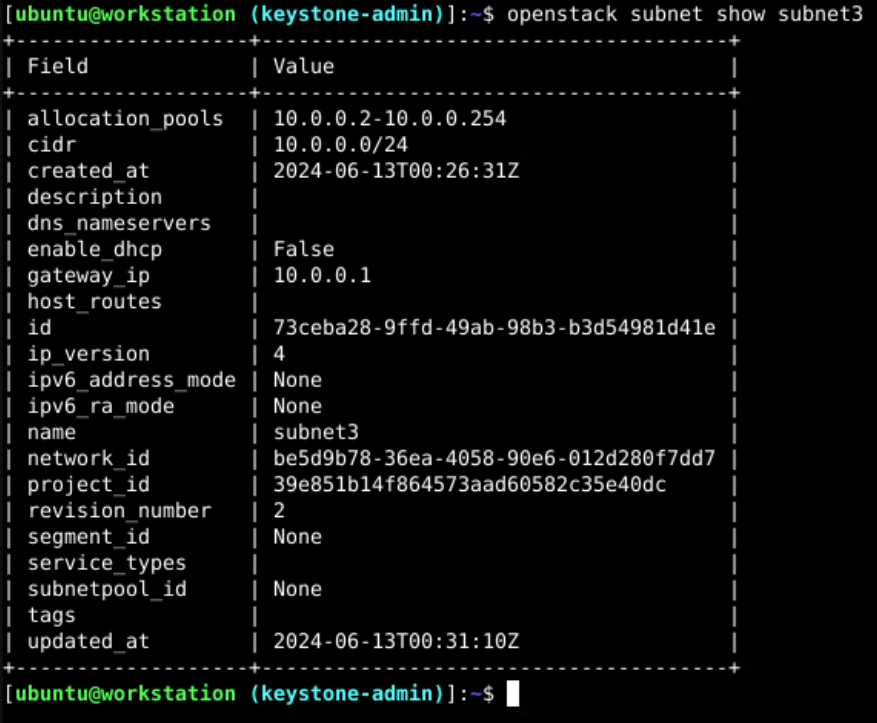
\includegraphics[width=\linewidth]{images/part3/step18.png}
    \end{center}

    \item To avoid confusion, also rename \textbf{subnet1} to \textbf{subnet3}.
    \begin{lstlisting}
        [ubuntu@workstation (keystone-admin)]:~$ openstack subnet set \
        > --name subnet3 subnet1
    \end{lstlisting}

    \begin{center}
        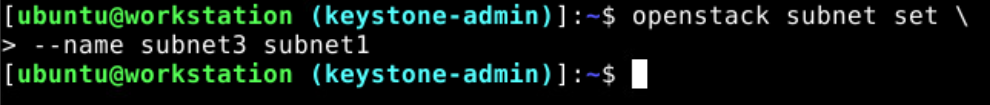
\includegraphics[width=\linewidth]{images/part3/step19.png}
    \end{center}

    \item Show the details of \textbf{subnet3}. Notice that DHCP is enabled for this subnet (\textbf{enable\_dhcp} is
    set to \textbf{True}).
    \begin{lstlisting}
        [ubuntu@workstation (keystone-admin)]:~$ openstack subnet show subnet3
    \end{lstlisting}

    \begin{center}
        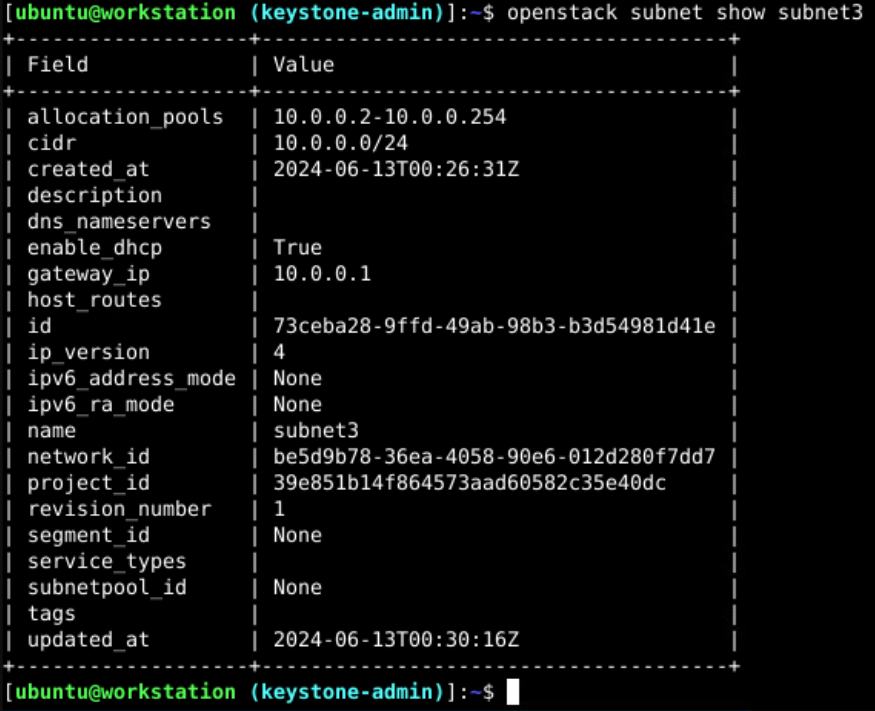
\includegraphics[width=\linewidth]{images/part3/step20.png}
    \end{center}

    \item Update the \textbf{subnet3} subnet to disable DHCP.
    \begin{lstlisting}
        [ubuntu@workstation (keystone-admin)]:~$ openstack subnet set \
        > --no-dhcp subnet3
    \end{lstlisting}

    \begin{center}
        \includegraphics[width=\linewidth]{images/part3/step21.png}
    \end{center}

    \item Verify that the \textbf{subnet3} subnetwork has been correctly updated.
    \begin{lstlisting}
        [ubuntu@workstation (keystone-admin)]:~$ openstack subnet show subnet3
    \end{lstlisting}

    \begin{center}
        \includegraphics[width=\linewidth]{images/part3/step22.png}
    \end{center}

    \item The \textbf{net3} network is now ready to be deleted, which will also delete its subnets. To confirm this,
    first list the current subnets.
    \begin{lstlisting}
        [ubuntu@workstation (keystone-admin)]:~$ openstack subnet list
    \end{lstlisting}

    \begin{center}
        \includegraphics[width=\linewidth]{images/part3/step23.png}
    \end{center}

    \item Delete the \textbf{net3} network.
    \begin{lstlisting}
        [ubuntu@workstation (keystone-admin)]:~$ openstack network delete net3
    \end{lstlisting}

    \begin{center}
        \includegraphics[width=\linewidth]{images/part3/step24.png}
    \end{center}

    \item Verify that the \textbf{net3} network has been deleted by listing all available networks and noting that
    \textbf{net3} is not present in the list.
    \begin{lstlisting}
        [ubuntu@workstation (keystone-admin)]:~$ openstack network list
    \end{lstlisting}

    \begin{center}
        \includegraphics[width=\linewidth]{images/part3/step25.png}
    \end{center}

    \item Verify that the subnet attached to the \textbf{net3} network was deleted along with the network.
    \begin{lstlisting}
        [ubuntu@workstation (keystone-admin)]:~$ openstack subnet list
    \end{lstlisting}

    \begin{center}
        \includegraphics[width=\linewidth]{images/part3/step26.png}
    \end{center}

    \item Leave the terminal window open and continue to the next task.

\end{enumerate}

%%%%%%%%%%%
% Section 4
%%%%%%%%%%%
\section{Launching an Internal Instance}
\label{sec:launching_an_internal_instance}
In this task, you will launch an internal instance with the \textit{Horizon Dashboard}. You will then delete that
instance and launch a new instance by using the \textit{Horizon Unified CLI}.

\begin{enumerate}
    \item Open the web browser and navigate to \textbf{192.168.1.20}. Login as the \textbf{admin} user with the password
    \textbf{secret}.

    \item Switch to the \textbf{demo} project and navigate to
    \textbf{Projects $>$ Compute $>$ Instances}. Click \textbf{Launch Instance}.

    \begin{center}
        \includegraphics[width=\linewidth]{images/part4/step2.png}
    \end{center}

    \item Ensure that \textbf{demo} is entered in the \textit{Project Name} field, and enter \textbf{instance1} in the
    \textit{Instance Name} field. Click \textbf{Next}.
    
    \begin{center}
        \includegraphics[width=\linewidth]{images/part4/step3.png}
    \end{center}

    \item Make sure \textbf{Image} is selected in the \textit{Select Boot Source} dropdown, and click \textbf{No} under
    \textit{Create New Volume}. Click the $\uparrow$ button on the same row as the \textbf{ubuntu2} image to allocate the
    image, and then click \textbf{Next}.

    \begin{center}
        \includegraphics[width=\linewidth]{images/part4/step4.png}
    \end{center}

    \begin{stopbox}
        Verify that \textbf{ubuntu2} appears in the \textit{Allocated} section before moving on to the next step.
    \end{stopbox}

    \item Click the $\uparrow$ button on the same row as the \textbf{flavor2} flavor to allocate that flavor, then
    click \textbf{Next}.
    \begin{center}
        \includegraphics[width=\linewidth]{images/part4/step5.png}
    \end{center}

    \begin{notebox}
        The warning signs in the \textit{Root Disk} column indicate that the flavor in that row has a disk size less
        than the minimum size specified for the selected image.
    \end{notebox}

    \item Click the $\uparrow$ button on the same row as the \textbf{net2} network, and click \textbf{Launch Instance}.

    \begin{center}
        \includegraphics[width=\linewidth]{images/part4/step6.png}
    \end{center}

    \begin{stopbox}
        Verify that \textbf{net2} appears under the \textit{Allocated} section. Wait for the instance to have a
        power state of \textbf{Running} before proceeding further.
    \end{stopbox}

    \item Log out of the \textit{Horizon Dashboard} and close the web browser.
    
    \item If a terminal window is not already open, open one and source the \textbf{\texttildemid/keystonerc-admin} file
    to load the \textbf{admin} user credentials.
    \begin{lstlisting}
        ubuntu@workstation:~$ source ~/keystonerc-admin        
    \end{lstlisting}

    \begin{center}
        \includegraphics[width=\linewidth]{images/part4/step8.png}
    \end{center}

    \item List the available instances and see that the instance created from the \textit{Horizon Dashboard} appears.
    \begin{lstlisting}
        [ubuntu@workstation (keystone-admin)]:~$ openstack server list
    \end{lstlisting}

    \begin{center}
        \includegraphics[width=\linewidth]{images/part4/step9.png}
    \end{center}

    \item Now, we will recreate the instance using the CLI. First, the \textbf{instance1} instance.
    \begin{lstlisting}
        [ubuntu@workstation (keystone-admin)]:~$ openstack server delete instance1
    \end{lstlisting}

    \begin{center}
        \includegraphics[width=\linewidth]{images/part4/step10.png}
    \end{center}

    \item List the instances again to verify that \textbf{instance1} was deleted successfully.
    \begin{lstlisting}
        [ubuntu@workstation (keystone-admin)]:~$ openstack server list
    \end{lstlisting}

    \begin{center}
        \includegraphics[width=\linewidth]{images/part4/step11.png}
    \end{center}

    \item Create a new instance named \textbf{instance2}. Use the previously created \textbf{ubuntu2} image,
    \textbf{flavor2} flavor, and \textbf{net2} network.
    \begin{lstlisting}
        [ubuntu@workstation (keystone-admin)]:~$ openstack server create \
        > --image ubuntu2 \
        > --flavor flavor2 \
        > --nic net-id=net2 \
        > instance2
    \end{lstlisting}

    \begin{center}
        \includegraphics[width=\linewidth]{images/part4/step12.png}
    \end{center}

    \item List all the available instance to verify that the \textbf{instance2} instance is running.
    \begin{lstlisting}
        [ubuntu@workstation (keystone-admin)]:~$ openstack server list
    \end{lstlisting}

    \begin{center}
        \includegraphics[width=\linewidth]{images/part4/step13.png}
    \end{center}

    \item Leave the terminal window open and continue to the next task.

\end{enumerate}

%%%%%%%%%%%
% Section 5
%%%%%%%%%%%
\section{Verifying the Functionality of an Internal Instance}
\label{sec:verifying_the_functionality_of_an_internal_instance}
In this task, you will connect to the instance and verify the flavor settings. You will also pause and stop an isntance
using the \textit{OpenStack Unified CLI}.

\begin{enumerate}
    \item If a terminal window is not already open, open one and source the \textbf{\texttildemid/keystonerc-admin} file
    to load the \textbf{admin} user credentials.
    \begin{lstlisting}
        ubuntu@workstation:~$ source ~/keystonerc-admin        
    \end{lstlisting}

    \begin{center}
        \includegraphics[width=\linewidth]{images/part5/step1.png}
    \end{center}

    \item List all the available instances to find the name of the running instance.
    \begin{lstlisting}
        [ubuntu@workstation (keystone-admin)]:~$ openstack server list
    \end{lstlisting}

    \begin{center}
        \includegraphics[width=\linewidth]{images/part5/step2.png}
    \end{center}

    \item Show more details of the instance.
    \begin{lstlisting}
        [ubuntu@workstation (keystone-admin)]:~$ openstack server show instance2
    \end{lstlisting}

    \begin{center}
        \includegraphics[width=\linewidth]{images/part5/step3.png}
    \end{center}

    \item Review the specifications of the \textbf{flavor2} flavor.
    \begin{lstlisting}
        [ubuntu@workstation (keystone-admin)]:~$ openstack flavor show flavor2
    \end{lstlisting}

    \begin{center}
        \includegraphics[width=\linewidth]{images/part5/step4.png}
    \end{center}

    \item Retrieve the URL for the noVNC console connection. Right click the link and select \textbf{Open Link}.
    \begin{lstlisting}
        [ubuntu@workstation (keystone-admin)]:~$ openstack console url show instance2
    \end{lstlisting}

    \begin{center}
        \includegraphics[width=\linewidth]{images/part5/step5.png}
    \end{center}

    \item Log in to the \textbf{instance2} instance as \textbf{root} with the password \textbf{secret}.
    
    \begin{center}
        \includegraphics[width=\linewidth]{images/part5/step6.png}
    \end{center}

    \item Use the \textbf{\texttt{free}} command to ensure that the RAM and swap amount matches the one defined by the
    flavor, which is \textbf{1024 MB} for each.
    \begin{lstlisting}
        root@instance2:~# free -m
    \end{lstlisting}

    \begin{center}
        \includegraphics[width=\linewidth]{images/part5/step7.png}
    \end{center}

    \item Use the \textbf{\texttt{df}} command to ensure that the instance has a disk size of \textbf{10 GB}, as defined
    by the flavor. Notice that \texttt{/dev/vda1} and \texttt{/dev/vdb} add up to almost 10 GB.
    \begin{lstlisting}
        root@instance2:~# df -h
    \end{lstlisting}

    \begin{center}
        \includegraphics[width=\linewidth]{images/part5/step8.png}
    \end{center}

    \item Determine the number of CPUs that the instance is using. Ensure the number matches the number of VCPUs defined
    by the flavor, which is \textbf{1}. Notice that under the \textbf{Architecture} heading at the top of the command
    output, there is a \textbf{CPU(s)} heading, whose value is 1.
    \begin{lstlisting}
        root@instance2:~# lscpu
    \end{lstlisting}

    \begin{center}
        \includegraphics[width=\linewidth]{images/part5/step9.png}
    \end{center}

    \item Use the \textbf{\texttt{ping}} command from the instance to reach the DHCP server defined for the network.
    Leave the \textbf{\texttt{ping}} command running, as it will be used in the following steps.
    \begin{lstlisting}
        root@instance2:~# ping -c3 192.168.1.2
    \end{lstlisting}

    \begin{center}
        \includegraphics[width=\linewidth]{images/part5/step10.png}
    \end{center}

    \begin{notebox}
        You should receive 3 successful ping replies.
    \end{notebox}

    \item Close the web browser and switch focus to the terminal on \textbf{workstation}.

    \item List the current OpenStack instances.
    \begin{lstlisting}
        [ubuntu@workstation (keystone-admin)]:~$ openstack server list
    \end{lstlisting}

    \begin{center}
        \includegraphics[width=\linewidth]{images/part5/step12.png}
    \end{center}

    \item Delete \textbf{instance2}.
    \begin{lstlisting}
        [ubuntu@workstation (keystone-admin)]:~$ openstack server delete instance2
    \end{lstlisting}

    \begin{center}
        \includegraphics[width=\linewidth]{images/part5/step13.png}
    \end{center}

    \item List all available instances to verify the \textbf{instance2} instance has been deleted.
    \begin{lstlisting}
        [ubuntu@workstation (keystone-admin)]:~$ openstack server list
    \end{lstlisting}

    \begin{center}
        \includegraphics[width=\linewidth]{images/part5/step14.png}
    \end{center}

    \item Close the terminal window and the web browser.
    
    \item The lab is now complete.

\end{enumerate}
\end{document}
